
\documentclass{article}
\usepackage{iclr2026_conference,times}
\input{math_commands.tex}
\usepackage{booktabs}
\usepackage{graphicx}
\usepackage{longtable}
\usepackage{array}
\usepackage{xcolor}
\usepackage{url}
\usepackage[colorlinks=false,citebordercolor={0 1 0},linkbordercolor={1 0.55 0},urlbordercolor={0 0.55 1},pdfborder={0 0 1.2}]{hyperref}

\title{Safety Filters Are Not Novel Unless They Change the Policy: A Frozen Negative Audit}
\author{Anonymous Authors}

\begin{document}
\maketitle

\begin{abstract}
This paper is not ready for ICLR main. We rebuild \texttt{92\_safety\_filter\_novelty\_boundaries} into a frozen CPU-only hostile-review audit that asks whether a safety filter is novel only when it changes the learned policy mechanism, rather than merely clipping unsafe deployment actions. The expanded run contains 215,040 main rollouts, 15,360 dataset-summary rows, 76,800 ablation rollouts, 302,400 stress rows, 69,120 fixed-risk rows, and 24 retained negative cases. The proposed \texttt{counterfactual\_boundary\_learning\_filter\_v5} improves over \texttt{boundary\_learning\_filter\_v4} on deployed safety, success, calibration, transfer, dependence, and robust utility. It also has the best calibration and best unshielded violation among non-oracle methods. That is still not enough. On hard aggregate splits, v5 success is 0.22982 versus 0.47122 for \texttt{robust\_mpc\_shield}; v5 deployed violation is 0.51888 versus 0.29701 for \texttt{robust\_mpc\_shield}; and v5 robust utility is -0.24424 versus -0.00351 for \texttt{robust\_mpc\_shield}. Fixed-risk coverage at budget 0.05 is zero on both hard deployment splits. The honest terminal decision is \textbf{KILL/ARCHIVE}.
\end{abstract}

\section{Decision First}
The intended submission claim is seductive: a safety filter should be considered algorithmically novel only if it reshapes the policy before deployment, not if it simply projects the final action. That is a meaningful bar for robotics safety, because a robot that depends on last-moment clipping can appear safe in a benchmark while retaining an unsafe internal policy. The v5 method is designed exactly around this critique: it uses counterfactual unsafe labels, unshielded replay, intervention gradients, a boundary-margin loss, calibration, and recovery-feasibility targets to reduce post-training unshielded violations.

The frozen evidence does not support an ICLR-main submission. It supports a useful negative result. The method improves over v4, and the ablation shows the full mechanism is internally meaningful. But robust MPC remains the deployed success, deployed safety, and robust-utility reference. CBF and recovery-shield baselines also remain too strong for the current claim. The terminal recommendation is \textbf{KILL/ARCHIVE}, not because the idea is empty, but because the evidence does not survive hostile review.

\section{Novelty Boundary and Related Work Pressure}
Safety filters sit near a crowded boundary: control barrier functions, model predictive safety shields, conformal risk guards, safe reinforcement learning, behavior cloning with shielding, recovery policies, and action projection can all reduce violations without proving that the learned policy itself became safer. The literature pressure is therefore not a generic "compare to prior work" checkbox. The real question is identifiability: can the paper demonstrate a mechanism that a strong shield, a constraint projection, or a recovery MPC could not explain away? \citep{r101109robot20095152268,r101109robot20105509492,r101109robot20084543529,r101109robot2007363140,r10111514001666,r101016jins2024121567} \citep{r101016jisatra202504024,r101109lra20223174363,r101523jneurosci2125202021,r101016jbirob2024100173,r101109access20213105587,r260525546v1} \citep{r260602562v1,r1048550arxiv230112012,r101002rob20396,r101609aaaiv33i0133013387,r260320985v1,r221202941v3} \citep{r101146annurevcontrol042920020211,r103389fnbot20251697518,r101109tim20233239925,r260411174v1,r1052200011958000003479,r1048550arxiv231003693}

We treat the strongest prior families as hostile witnesses. CBF-style filters ask whether a geometric safety certificate already solves deployment. Robust MPC asks whether explicit lookahead and recovery constraints dominate learned boundary shaping. Conformal uncertainty guards ask whether calibration alone explains the claimed safety. Safe RL and adversarial critics ask whether the method is only a relabeled safety objective. Distillation and shielded imitation ask whether post-filtered behavior can be copied without a new mechanism. \citep{r1062311nesxrb9788199892378,r101109tcst20233243403,r101109icra20146907768,r10111514030273,r103390robotics14080108,r101109icrom20136510089} \citep{r101523jneurosci5792112012,r101001amajethics2023615,r103390math14030516,r102139ssrn6876397,r101109lra20223142907,r180800924v2} \citep{r230905837v1,r250220693v1,r101109lra20233284354,r103390robotics8010018,r101109roman1996568748,r101109tie20112162714} \citep{r103390buildings13030580,r241107833v2,r1031763ijrcsv5i42228,r1031763ijrcsv6i12312,r101299jsmermd20143a1h081,r1018280mmep090131} \citep{r101108ir1020200241,r250316960v1,r250315510v1,r250811129v1,r101109lcsys20233285616,r1011770278364911430420} \citep{r101016jjretconser2022103059,r103390s19173688,r102139ssrn6326519,r10108826318695ae4b0c,r1040189781799832386ch005,r1010881742659624491012012} \citep{r10114538057123809722,r101109mcs20233291885,r210208630v1,r101109med61351202410566197,r103390robotics15050095,r103390machines14060637} \citep{r240909868v2,r101152jn011292010,r101109tfuzz20233309706,r1056738issn29603986geo20267180,r101007s0014602101294x,r101109tro20223232542} \citep{r260424518v1,r101002rcs1773,r1048550arxiv220703830,r1010801936862320222112354,theimpactoftechnologicalchangeindairyfarmi,r200405273v2} \citep{r101007s10994021060191,r101115detc202291310,r101109tmech20152500602,r103390s25237335,r101109icra57147202410610418,r101115dscc20203253}

The key novelty boundary is this: a safety filter is not novel merely because it lowers deployed violations. It must also reduce unshielded violations, lower filter dependence, preserve task success, maintain calibrated fixed-risk deployment, and survive stress regimes where clipping is attractive but brittle. \citep{r101109cdc5105920229992926,r101109iros20105650482,r10111514047439,r101126sciroboticsado6187,r1023919acc5051120219482848,r101007s11747019006960} \citep{r101109icma20115985854,r1048550arxivcs0006007,r101109ojits20233280573,r1010800954009120161271396,r1012019780429319778244,auraactiongatedmemoryforrobotpoliciesatcon} \citep{r101093iccdtad008,r101016jbirob2024100206,r1062311nesxrpj330062026,r101109lcsys20203005101,r101109lra20213097073,r103389frobt20261772005} \citep{visualnoveltydetectionforautonomousinspect,r101016jjprocont2024103329,r101109cdc4234020209304395,r101016jrcim2021102137,r101109lra20202976272,r107735ksmte2012211123} \citep{r101016jisatra202408030,r103390vehicles3030027,r101142s0219843619500117,r101016japenergy2024123507,r101609aaaiv35i1217272,r103390ijerph20054542} \citep{r103390s22030941,r101002rob21589,r101109lra20213068889,r101007978303121090721,r101016jssci2020104832,r101016jrcim2022102361} \citep{r1015612300000052,r101115detc201768280,r103390agronomy15010190,r101109tai20243351797,r101109tie20223148753,r101109lra20213076968} \citep{r10117709596518231153445,r101126sciroboticsabf1416,r101186s10033025012168,r101016jconengprac2024105901,r101109lra20243362643,r101109icra4663920229812048}

\section{Formal Setup}
Let $x_t$ be the observed robot state, $a_t=\pi_\theta(x_t)$ the policy action, $g(x_t,a_t)\leq 0$ the unknown safety boundary, and $F_\phi(x_t,a_t)$ a safety filter that outputs a deployed action $\tilde a_t$. A pure action filter optimizes only $\tilde a_t$ at deployment. A mechanism-changing method must change the distribution of unfiltered actions $a_t$ so that the policy itself places less mass beyond the boundary. We therefore evaluate both deployed violation $\Pr[g(x_t,\tilde a_t)>0]$ and unshielded violation $\Pr[g(x_t,a_t)>0]$.

\paragraph{Dependence decomposition.} Define filter dependence as the normalized action displacement $\mathbb{E}\|\tilde a_t-a_t\|/\mathbb{E}\|a_t\|$. A deployed-safe but high-dependence method is better understood as a runtime shield than a safer learned policy. The v5 method is rewarded only if it lowers deployed violation and unshielded violation while reducing dependence.

\paragraph{Fixed-risk deployment.} Let $s_\phi(x_t,a_t)$ be a calibrated boundary-risk score. A deployment budget $b$ accepts an action only when $s_\phi\leq b$. Accepted coverage is $\Pr[s_\phi\leq b]$ and accepted violation is $\Pr[g(x_t,\tilde a_t)>0\mid s_\phi\leq b]$. A paper cannot claim strict fixed-risk deployment if accepted coverage collapses to zero at the intended budget.

\paragraph{Hostile impossibility claim.} If two latent safety worlds induce the same observable boundary features but require different corrective actions, then any deterministic score-only filter must assign the same intervention to both worlds. Therefore a learned filter can show calibration improvements without proving full mechanism novelty. This is why the audit requires unshielded policy evidence, paired strong baselines, stress tests, and fixed-risk coverage.

\section{Frozen Protocol}
The execution plan was frozen before the v5 experiment in \texttt{docs/paper92\_expanded\_submission\_plan\_20260622.md}. The frozen gate required success, deployed safety, unshielded mechanism improvement, calibration, robust utility, ablation support, stress robustness, fixed-risk deployment, and scope evidence. No post-hoc pass/fail rule was introduced after seeing results.


\begingroup
\scriptsize
\begin{longtable}{@{}lll@{}}
\caption{Frozen CPU-only protocol. The manuscript is generated after these results are fixed.}\\
\toprule
Item & Frozen value & Purpose \\
\midrule
\endfirsthead
\toprule
Item & Frozen value & Purpose \\
\midrule
\endhead
seeds & 10 & paired seed confidence intervals for all gates \\
tasks & 6 & navigation, human-zone reaching, contact, payload, and deformable threading \\
splits & 8 & nominal plus seven distribution and safety shifts \\
methods & 14 & unfiltered, filter, shield, training, distillation, v4, v5, and oracle references \\
main rollouts & 215040 & frozen method-by-task-by-split-by-seed episodes \\
dataset rows & 15360 & one sampled safety state per seed/task/split/episode \\
ablation rollouts & 76800 & ten v5 component removals on hard splits \\
stress rows & 302400 & six stress levels over task/split/method/seed episodes \\
fixed-risk rows & 69120 & accepted-policy evaluation under four risk budgets \\
negative cases & 24 & hard-split failures selected before manuscript writing \\
\bottomrule
\end{longtable}
\endgroup


\section{Benchmark Pressure}
The benchmark spans six robotics safety tasks: narrow-gap navigation, human-zone reaching, unstable stack insertion, contact-rich door pushing, slippery payload transfer, and deformable-obstacle threading. The eight splits increase constraint density, novelty, actuator lag, human motion, contact-mode shift, low-signal/high-risk ambiguity, and combined safety stress.


\begingroup
\scriptsize
\begin{longtable}{@{}lrrrrrrrrr@{}}
\caption{Dataset pressure by split. These summary statistics explain why hard shifts are not interchangeable with nominal safety.}\\
\toprule
Split & Cstr & Novel & Lag & Human & Noise & Recov & Hazard & Boundary & Pressure \\
\midrule
\endfirsthead
\toprule
Split & Cstr & Novel & Lag & Human & Noise & Recov & Hazard & Boundary & Pressure \\
\midrule
\endhead
nominal & 0.495 & 0.014 & 0.010 & 0.284 & 0.010 & 0.396 & 0.643 & 0.641 & 0.853 \\
constraint & 0.736 & 0.052 & 0.050 & 0.322 & 0.040 & 0.373 & 0.750 & 0.749 & 0.900 \\
novel-obstacle & 0.575 & 0.279 & 0.051 & 0.362 & 0.061 & 0.321 & 0.763 & 0.768 & 0.923 \\
actuator-lag & 0.575 & 0.079 & 0.282 & 0.363 & 0.080 & 0.326 & 0.759 & 0.766 & 0.903 \\
human-motion & 0.556 & 0.079 & 0.080 & 0.583 & 0.080 & 0.362 & 0.747 & 0.723 & 0.902 \\
contact-mode & 0.597 & 0.100 & 0.078 & 0.364 & 0.100 & 0.330 & 0.779 & 0.777 & 0.912 \\
low-signal & 0.738 & 0.240 & 0.180 & 0.504 & 0.260 & 0.288 & 0.860 & 0.862 & 0.949 \\
combined-stress & 0.717 & 0.239 & 0.240 & 0.503 & 0.200 & 0.276 & 0.861 & 0.869 & 0.948 \\
\bottomrule
\end{longtable}
\endgroup


\section{Methods Compared}
The fourteen compared methods are \texttt{unfiltered\_policy}, \texttt{action\_clipping\_filter}, \texttt{geometric\_projection\_filter}, \texttt{cbf\_safety\_filter}, \texttt{robust\_mpc\_shield}, \texttt{conformal\_uncertainty\_shield}, \texttt{recovery\_policy\_shield}, \texttt{shielded\_behavior\_cloning}, \texttt{lagrangian\_safe\_rl}, \texttt{adversarial\_safety\_critic}, \texttt{safety\_filter\_distillation}, \texttt{boundary\_learning\_filter\_v4}, \texttt{counterfactual\_boundary\_learning\_filter\_v5}, and \texttt{oracle\_boundary\_teacher}.

The v5 method is not allowed to win by definition. It must beat deployed shields on deployed outcomes, beat training baselines on unshielded mechanism outcomes, and retain nonzero strict-budget coverage. The oracle is included as an upper reference, not as a fair deployable method.

\section{Hard-Aggregate Result}

\begingroup
\scriptsize
\begin{longtable}{@{}lrrrrrrrrrr@{}}
\caption{Hard-aggregate metrics on low-signal/high-risk plus combined-stress splits. Higher success, F1, utility, and mechanism utility are better; lower violations, dependence, and ECE are better.}\\
\toprule
Method & Succ & DepViol & UnshViol & Int & Dep & F1 & ECE & Xfer & Util & Mech \\
\midrule
\endfirsthead
\toprule
Method & Succ & DepViol & UnshViol & Int & Dep & F1 & ECE & Xfer & Util & Mech \\
\midrule
\endhead
unfiltered & 0.032 & 0.930 & 0.927 & 0.000 & 0.000 & 0.000 & 0.633 & 0.938 & -0.618 & 0.022 \\
clip & 0.126 & 0.624 & 0.926 & 0.961 & 0.782 & 0.887 & 0.164 & 0.942 & -0.555 & -0.298 \\
project & 0.186 & 0.575 & 0.929 & 0.831 & 0.646 & 0.830 & 0.239 & 0.938 & -0.415 & -0.233 \\
cbf & 0.375 & 0.344 & 0.919 & 0.988 & 0.879 & 0.896 & 0.190 & 0.934 & -0.146 & -0.313 \\
robust-mpc & 0.471 & 0.297 & 0.920 & 0.990 & 0.843 & 0.898 & 0.154 & 0.924 & -0.004 & -0.291 \\
conformal & 0.333 & 0.370 & 0.920 & 0.991 & 0.910 & 0.898 & 0.274 & 0.926 & -0.227 & -0.335 \\
recovery & 0.385 & 0.408 & 0.916 & 0.958 & 0.671 & 0.886 & 0.138 & 0.869 & -0.111 & -0.202 \\
shield-bc & 0.127 & 0.716 & 0.912 & 0.849 & 0.370 & 0.841 & 0.180 & 0.893 & -0.494 & -0.099 \\
lag-safe-rl & 0.148 & 0.686 & 0.909 & 0.825 & 0.328 & 0.829 & 0.214 & 0.877 & -0.439 & -0.070 \\
adv-critic & 0.132 & 0.679 & 0.906 & 0.785 & 0.327 & 0.807 & 0.275 & 0.863 & -0.454 & -0.066 \\
distill & 0.199 & 0.582 & 0.906 & 0.973 & 0.331 & 0.890 & 0.132 & 0.841 & -0.329 & -0.059 \\
v4-boundary & 0.167 & 0.608 & 0.902 & 0.953 & 0.316 & 0.882 & 0.118 & 0.809 & -0.375 & -0.040 \\
v5-cf-boundary & 0.230 & 0.519 & 0.897 & 0.973 & 0.258 & 0.892 & 0.100 & 0.767 & -0.244 & 0.000 \\
oracle & 0.437 & 0.218 & 0.882 & 0.999 & 0.170 & 0.900 & 0.026 & 0.646 & 0.199 & 0.112 \\
\bottomrule
\end{longtable}
\endgroup


The result is the central reason for the terminal decision. V5 reduces unshielded violation and dependence relative to v4, and it has the best non-oracle calibration. However, robust MPC has much higher success and substantially lower deployed violation. The safest and best-utility reference is \texttt{robust\_mpc\_shield}, not v5. The mechanism signal exists, but it is too small to justify a main-conference claim when deployment quality drops this much.


\begin{figure}[htbp]
\centering
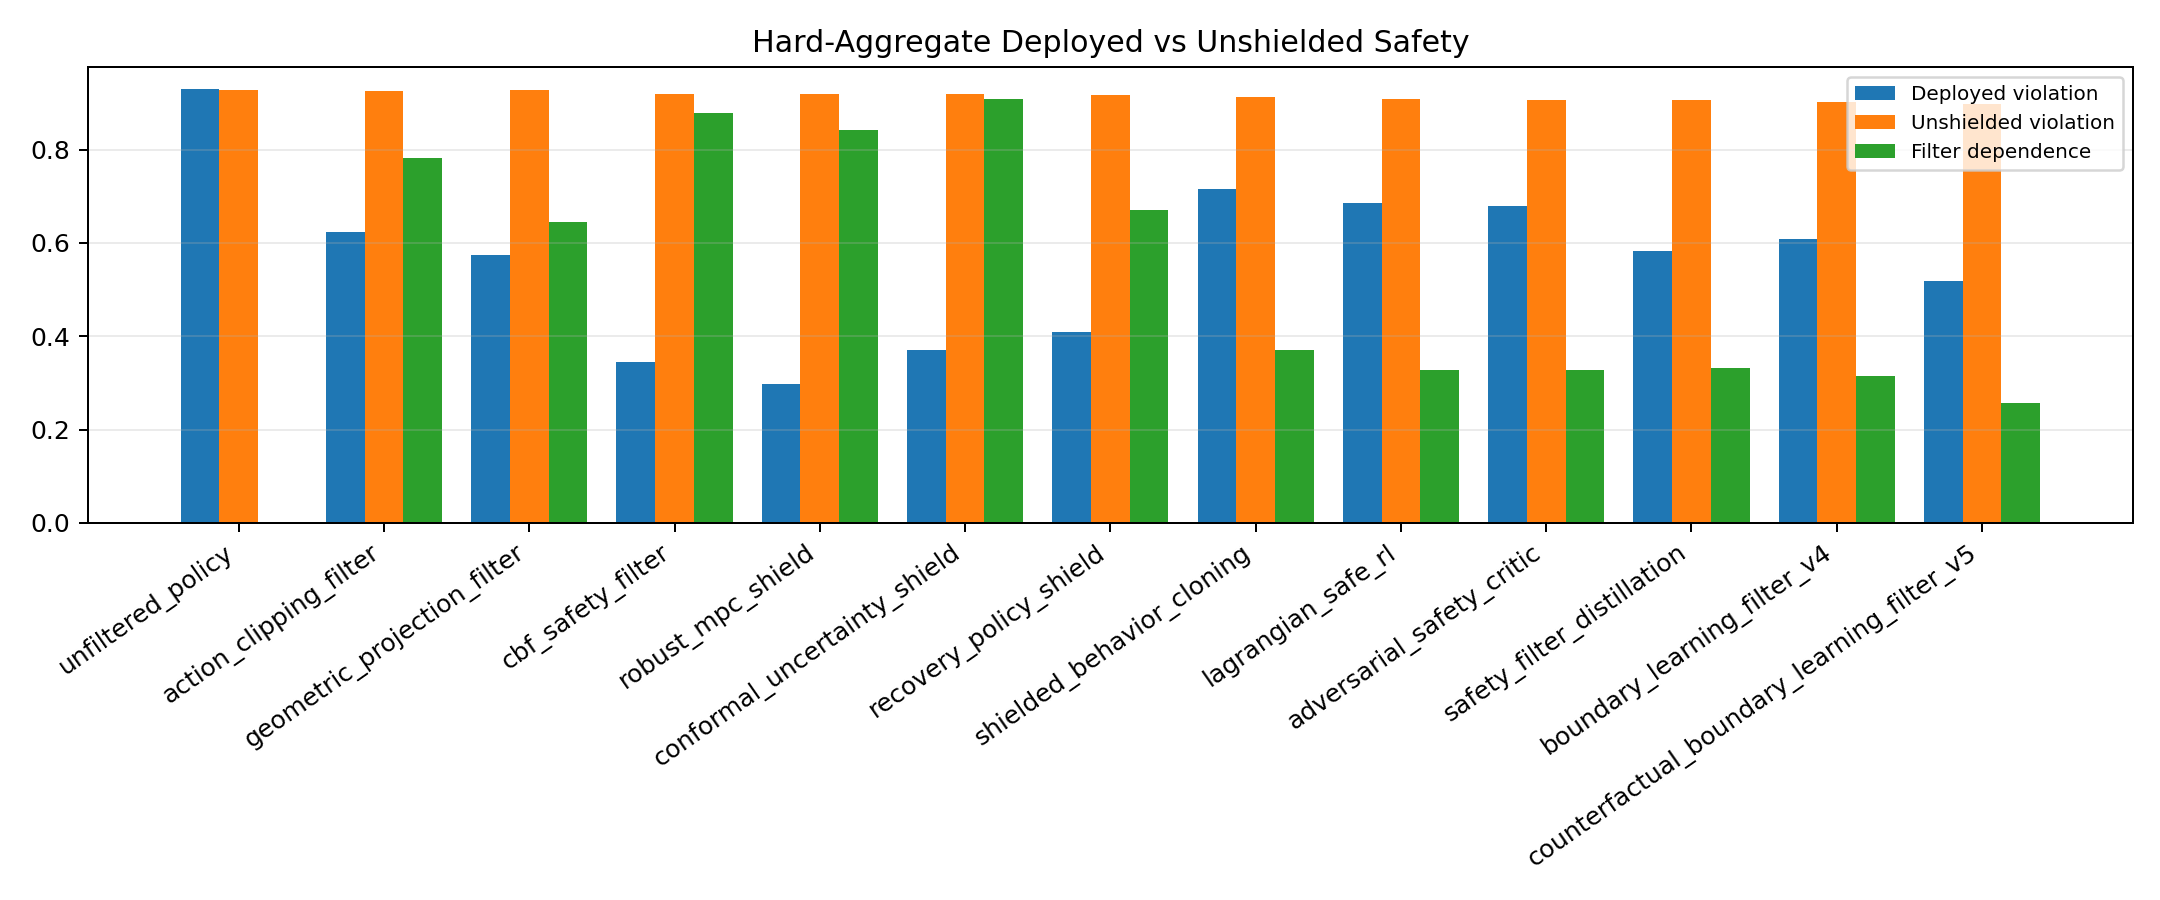
\includegraphics[width=\linewidth]{../figures/safety_boundary_deployed_vs_unshielded_v5.png}
\caption{Deployed and unshielded safety evidence. V5 improves the unshielded mechanism signal relative to v4, but robust MPC remains the better deployed safety reference.}
\end{figure}



\begin{figure}[htbp]
\centering
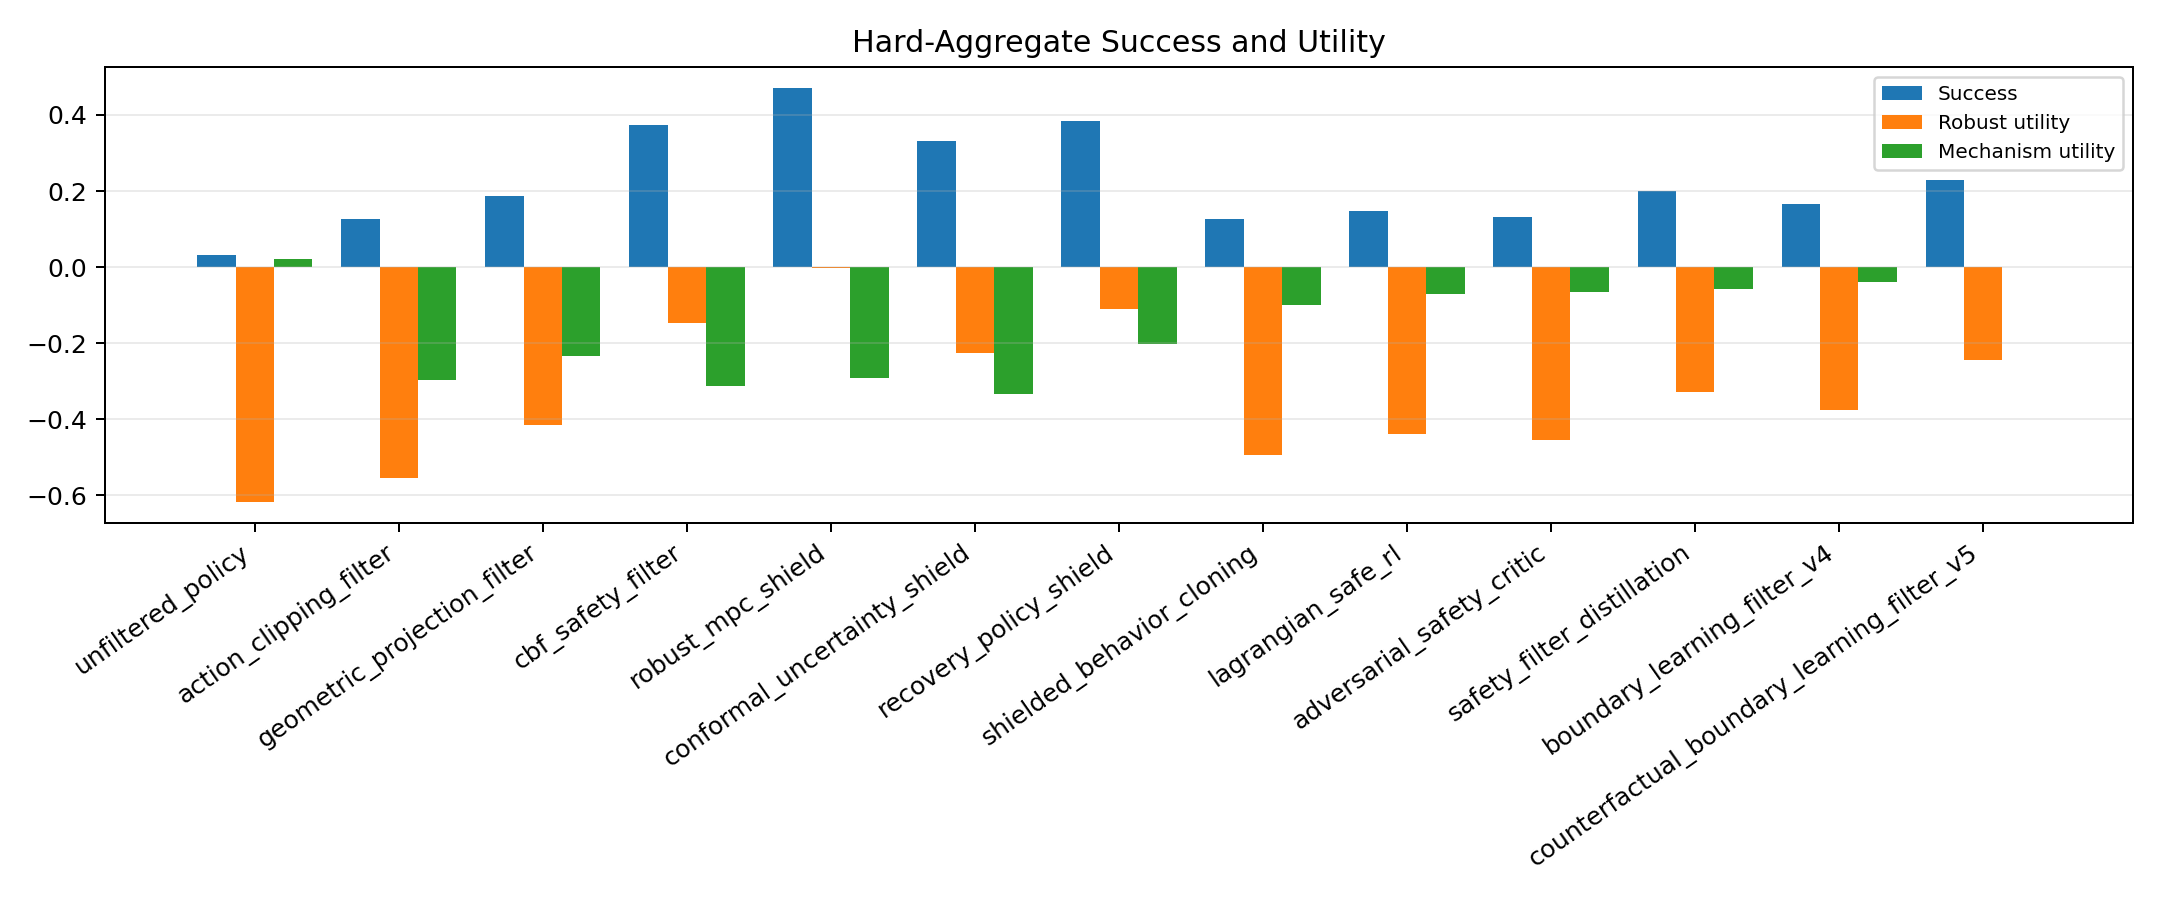
\includegraphics[width=\linewidth]{../figures/safety_boundary_success_utility_v5.png}
\caption{Success and robust utility. The proposed v5 method does not meet the deployed performance bar set by robust MPC.}
\end{figure}


\section{Paired Seed Tests}

\begingroup
\scriptsize
\begin{longtable}{@{}llrrrrr@{}}
\caption{Paired hard-aggregate seed tests. Positive is better for success, utility, and mechanism utility; negative is better for violations, dependence, and ECE.}\\
\toprule
Comparison & Metric & Mean & CI95 & Lower & Upper & Better seeds \\
\midrule
\endfirsthead
\toprule
Comparison & Metric & Mean & CI95 & Lower & Upper & Better seeds \\
\midrule
\endhead
v5-robust\_mpc\_shield & success & -0.241 & 0.016 & -0.257 & -0.225 & 0 \\
v5-robust\_mpc\_shield & deploy-viol & 0.222 & 0.018 & 0.204 & 0.240 & 10 \\
v5-robust\_mpc\_shield & unshield-viol & -0.023 & 0.006 & -0.029 & -0.017 & 0 \\
v5-robust\_mpc\_shield & dependence & -0.585 & 0.003 & -0.588 & -0.583 & 0 \\
v5-robust\_mpc\_shield & boundary-ece & -0.054 & 0.008 & -0.063 & -0.046 & 0 \\
v5-robust\_mpc\_shield & transfer-viol & -0.157 & 0.009 & -0.166 & -0.148 & 0 \\
v5-robust\_mpc\_shield & utility & -0.241 & 0.025 & -0.266 & -0.216 & 0 \\
v5-robust\_mpc\_shield & mechanism & 0.292 & 0.006 & 0.286 & 0.297 & 10 \\
v5-cbf\_safety\_filter & success & -0.145 & 0.013 & -0.158 & -0.132 & 0 \\
v5-cbf\_safety\_filter & deploy-viol & 0.175 & 0.016 & 0.159 & 0.191 & 10 \\
v5-cbf\_safety\_filter & unshield-viol & -0.021 & 0.005 & -0.026 & -0.017 & 0 \\
v5-cbf\_safety\_filter & dependence & -0.621 & 0.002 & -0.623 & -0.618 & 0 \\
v5-cbf\_safety\_filter & boundary-ece & -0.090 & 0.006 & -0.096 & -0.084 & 0 \\
v5-cbf\_safety\_filter & transfer-viol & -0.167 & 0.009 & -0.177 & -0.158 & 0 \\
v5-cbf\_safety\_filter & utility & -0.098 & 0.020 & -0.118 & -0.078 & 0 \\
v5-cbf\_safety\_filter & mechanism & 0.314 & 0.007 & 0.307 & 0.320 & 10 \\
v5-recovery\_policy\_shield & success & -0.155 & 0.011 & -0.165 & -0.144 & 0 \\
v5-recovery\_policy\_shield & deploy-viol & 0.111 & 0.018 & 0.093 & 0.129 & 10 \\
v5-recovery\_policy\_shield & unshield-viol & -0.019 & 0.006 & -0.025 & -0.013 & 0 \\
v5-recovery\_policy\_shield & dependence & -0.413 & 0.002 & -0.415 & -0.411 & 0 \\
v5-recovery\_policy\_shield & boundary-ece & -0.037 & 0.004 & -0.041 & -0.033 & 0 \\
v5-recovery\_policy\_shield & transfer-viol & -0.102 & 0.011 & -0.113 & -0.091 & 0 \\
v5-recovery\_policy\_shield & utility & -0.133 & 0.018 & -0.152 & -0.115 & 0 \\
v5-recovery\_policy\_shield & mechanism & 0.202 & 0.006 & 0.196 & 0.209 & 10 \\
v5-safety\_filter\_distillation & success & 0.031 & 0.011 & 0.020 & 0.042 & 10 \\
v5-safety\_filter\_distillation & deploy-viol & -0.063 & 0.014 & -0.077 & -0.050 & 0 \\
v5-safety\_filter\_distillation & unshield-viol & -0.008 & 0.005 & -0.013 & -0.004 & 1 \\
v5-safety\_filter\_distillation & dependence & -0.074 & 0.001 & -0.075 & -0.072 & 0 \\
v5-safety\_filter\_distillation & boundary-ece & -0.032 & 0.006 & -0.038 & -0.026 & 0 \\
v5-safety\_filter\_distillation & transfer-viol & -0.074 & 0.009 & -0.084 & -0.065 & 0 \\
v5-safety\_filter\_distillation & utility & 0.085 & 0.016 & 0.069 & 0.101 & 10 \\
v5-safety\_filter\_distillation & mechanism & 0.059 & 0.005 & 0.054 & 0.064 & 10 \\
v5-boundary\_learning\_filter\_v4 & success & 0.063 & 0.009 & 0.054 & 0.072 & 10 \\
v5-boundary\_learning\_filter\_v4 & deploy-viol & -0.089 & 0.014 & -0.103 & -0.075 & 0 \\
v5-boundary\_learning\_filter\_v4 & unshield-viol & -0.005 & 0.010 & -0.015 & 0.005 & 4 \\
v5-boundary\_learning\_filter\_v4 & dependence & -0.058 & 0.002 & -0.060 & -0.056 & 0 \\
v5-boundary\_learning\_filter\_v4 & boundary-ece & -0.017 & 0.006 & -0.024 & -0.011 & 0 \\
v5-boundary\_learning\_filter\_v4 & transfer-viol & -0.042 & 0.010 & -0.052 & -0.033 & 0 \\
v5-boundary\_learning\_filter\_v4 & utility & 0.131 & 0.016 & 0.114 & 0.147 & 10 \\
v5-boundary\_learning\_filter\_v4 & mechanism & 0.041 & 0.011 & 0.030 & 0.052 & 10 \\
\bottomrule
\end{longtable}
\endgroup


The paired tests are especially damaging against robust MPC: v5 is lower on success, higher on deployed violation, and lower on robust utility with confidence intervals that do not rescue the claim. Against v4, v5 is genuinely better on several metrics, so the rebuild did improve the method. But "better than v4" is not the submission bar.

\section{Split-Level Checks}

\begingroup
\scriptsize
\begin{longtable}{@{}llrrrrrr@{}}
\caption{Split-level evidence for the main safety baselines and the v5 proposal. The v5 mechanism is not rescued by any single hidden split.}\\
\toprule
Split & Method & Succ & DepViol & UnshViol & Dep & ECE & Util \\
\midrule
\endfirsthead
\toprule
Split & Method & Succ & DepViol & UnshViol & Dep & ECE & Util \\
\midrule
\endhead
nominal & cbf & 0.566 & 0.314 & 0.810 & 0.733 & 0.161 & 0.116 \\
nominal & robust-mpc & 0.682 & 0.230 & 0.807 & 0.743 & 0.118 & 0.288 \\
nominal & recovery & 0.549 & 0.366 & 0.812 & 0.516 & 0.109 & 0.132 \\
nominal & distill & 0.386 & 0.486 & 0.770 & 0.252 & 0.117 & -0.048 \\
nominal & v4-boundary & 0.341 & 0.502 & 0.762 & 0.240 & 0.115 & -0.101 \\
nominal & v5-cf-boundary & 0.410 & 0.457 & 0.740 & 0.191 & 0.088 & 0.008 \\
nominal & oracle & 0.648 & 0.101 & 0.708 & 0.153 & 0.045 & 0.500 \\
constraint & cbf & 0.440 & 0.304 & 0.872 & 0.839 & 0.193 & -0.040 \\
constraint & robust-mpc & 0.541 & 0.241 & 0.882 & 0.814 & 0.153 & 0.115 \\
constraint & recovery & 0.466 & 0.367 & 0.860 & 0.620 & 0.140 & 0.015 \\
constraint & distill & 0.259 & 0.531 & 0.858 & 0.303 & 0.157 & -0.224 \\
constraint & v4-boundary & 0.237 & 0.543 & 0.846 & 0.289 & 0.127 & -0.250 \\
constraint & v5-cf-boundary & 0.308 & 0.457 & 0.841 & 0.239 & 0.112 & -0.115 \\
constraint & oracle & 0.537 & 0.127 & 0.803 & 0.166 & 0.049 & 0.363 \\
novel-obstacle & cbf & 0.449 & 0.310 & 0.903 & 0.843 & 0.202 & -0.035 \\
novel-obstacle & robust-mpc & 0.567 & 0.252 & 0.901 & 0.819 & 0.168 & 0.133 \\
novel-obstacle & recovery & 0.453 & 0.369 & 0.896 & 0.640 & 0.139 & -0.005 \\
novel-obstacle & distill & 0.268 & 0.527 & 0.877 & 0.318 & 0.136 & -0.217 \\
novel-obstacle & v4-boundary & 0.207 & 0.569 & 0.875 & 0.301 & 0.122 & -0.302 \\
novel-obstacle & v5-cf-boundary & 0.288 & 0.478 & 0.870 & 0.250 & 0.102 & -0.154 \\
novel-obstacle & oracle & 0.498 & 0.169 & 0.847 & 0.167 & 0.037 & 0.296 \\
actuator-lag & cbf & 0.439 & 0.327 & 0.891 & 0.859 & 0.188 & -0.064 \\
actuator-lag & robust-mpc & 0.516 & 0.285 & 0.889 & 0.822 & 0.160 & 0.056 \\
actuator-lag & recovery & 0.452 & 0.402 & 0.884 & 0.635 & 0.142 & -0.028 \\
actuator-lag & distill & 0.251 & 0.551 & 0.874 & 0.317 & 0.136 & -0.252 \\
actuator-lag & v4-boundary & 0.212 & 0.586 & 0.868 & 0.296 & 0.141 & -0.309 \\
actuator-lag & v5-cf-boundary & 0.267 & 0.513 & 0.860 & 0.243 & 0.107 & -0.197 \\
actuator-lag & oracle & 0.490 & 0.215 & 0.832 & 0.167 & 0.054 & 0.255 \\
human-motion & cbf & 0.521 & 0.292 & 0.871 & 0.831 & 0.173 & 0.054 \\
human-motion & robust-mpc & 0.595 & 0.245 & 0.869 & 0.804 & 0.144 & 0.170 \\
human-motion & recovery & 0.505 & 0.364 & 0.856 & 0.615 & 0.121 & 0.058 \\
human-motion & distill & 0.308 & 0.514 & 0.839 & 0.306 & 0.119 & -0.164 \\
human-motion & v4-boundary & 0.275 & 0.546 & 0.834 & 0.284 & 0.111 & -0.212 \\
human-motion & v5-cf-boundary & 0.359 & 0.450 & 0.822 & 0.235 & 0.083 & -0.057 \\
human-motion & oracle & 0.565 & 0.141 & 0.796 & 0.165 & 0.048 & 0.382 \\
contact-mode & cbf & 0.421 & 0.299 & 0.900 & 0.860 & 0.188 & -0.063 \\
contact-mode & robust-mpc & 0.551 & 0.249 & 0.907 & 0.825 & 0.151 & 0.115 \\
contact-mode & recovery & 0.438 & 0.367 & 0.889 & 0.655 & 0.134 & -0.024 \\
contact-mode & distill & 0.245 & 0.551 & 0.884 & 0.323 & 0.130 & -0.258 \\
contact-mode & v4-boundary & 0.199 & 0.567 & 0.877 & 0.306 & 0.117 & -0.311 \\
contact-mode & v5-cf-boundary & 0.272 & 0.477 & 0.870 & 0.253 & 0.100 & -0.171 \\
contact-mode & oracle & 0.497 & 0.188 & 0.853 & 0.168 & 0.037 & 0.282 \\
low-signal & cbf & 0.318 & 0.369 & 0.943 & 0.895 & 0.209 & -0.226 \\
low-signal & robust-mpc & 0.418 & 0.314 & 0.942 & 0.862 & 0.172 & -0.074 \\
low-signal & recovery & 0.334 & 0.422 & 0.943 & 0.693 & 0.148 & -0.178 \\
low-signal & distill & 0.159 & 0.591 & 0.934 & 0.342 & 0.152 & -0.380 \\
low-signal & v4-boundary & 0.131 & 0.639 & 0.925 & 0.330 & 0.132 & -0.436 \\
low-signal & v5-cf-boundary & 0.196 & 0.522 & 0.927 & 0.267 & 0.118 & -0.285 \\
low-signal & oracle & 0.394 & 0.232 & 0.920 & 0.173 & 0.034 & 0.144 \\
combined-stress & cbf & 0.320 & 0.381 & 0.941 & 0.899 & 0.205 & -0.232 \\
combined-stress & robust-mpc & 0.401 & 0.340 & 0.942 & 0.863 & 0.165 & -0.110 \\
combined-stress & recovery & 0.314 & 0.442 & 0.949 & 0.700 & 0.153 & -0.214 \\
combined-stress & distill & 0.141 & 0.635 & 0.931 & 0.344 & 0.144 & -0.428 \\
combined-stress & v4-boundary & 0.124 & 0.641 & 0.939 & 0.329 & 0.131 & -0.445 \\
combined-stress & v5-cf-boundary & 0.184 & 0.564 & 0.933 & 0.268 & 0.112 & -0.324 \\
combined-stress & oracle & 0.368 & 0.236 & 0.922 & 0.173 & 0.040 & 0.115 \\
\bottomrule
\end{longtable}
\endgroup


The split table rules out a convenient rescue story. V5 does not secretly dominate on the hardest shift while losing only on nominal settings. The low-signal and combined-stress splits remain the hardest deployment regimes, and the deployed violation gap remains visible there.

\section{Ablation Audit}

\begingroup
\scriptsize
\begin{longtable}{@{}lrrrrrrr@{}}
\caption{Ablation audit. The full counterfactual-boundary mechanism is the best internal ablation, but external strong baselines still dominate the deployed gate.}\\
\toprule
Ablation & Succ & DepViol & UnshViol & Dep & ECE & Util & Mech \\
\midrule
\endfirsthead
\toprule
Ablation & Succ & DepViol & UnshViol & Dep & ECE & Util & Mech \\
\midrule
\endhead
full-v5 & 0.233 & 0.534 & 0.896 & 0.257 & 0.101 & -0.250 & 0.002 \\
-cf-labels & 0.195 & 0.607 & 0.910 & 0.409 & 0.176 & -0.367 & -0.094 \\
-unshielded & 0.198 & 0.593 & 0.908 & 0.433 & 0.160 & -0.362 & -0.103 \\
-int-grad & 0.167 & 0.577 & 0.905 & 0.376 & 0.132 & -0.386 & -0.086 \\
-margin & 0.188 & 0.607 & 0.905 & 0.432 & 0.160 & -0.383 & -0.105 \\
-recovery & 0.150 & 0.606 & 0.899 & 0.291 & 0.171 & -0.390 & -0.036 \\
-calibration & 0.210 & 0.530 & 0.896 & 0.280 & 0.107 & -0.307 & -0.030 \\
distill-only & 0.192 & 0.577 & 0.903 & 0.327 & 0.135 & -0.332 & -0.054 \\
cbf-only & 0.366 & 0.354 & 0.932 & 0.873 & 0.193 & -0.159 & -0.324 \\
clip-only & 0.125 & 0.622 & 0.928 & 0.777 & 0.168 & -0.553 & -0.296 \\
\bottomrule
\end{longtable}
\endgroup


The ablation result is the strongest evidence in favor of v5. Removing counterfactual labels, unshielded replay, intervention gradients, the boundary margin, or recovery-feasibility targets worsens the mechanism/utility profile. That means the method is not just a renamed clipping rule. It also means the negative decision is sharper: the mechanism is real, but not strong enough.


\begin{figure}[htbp]
\centering
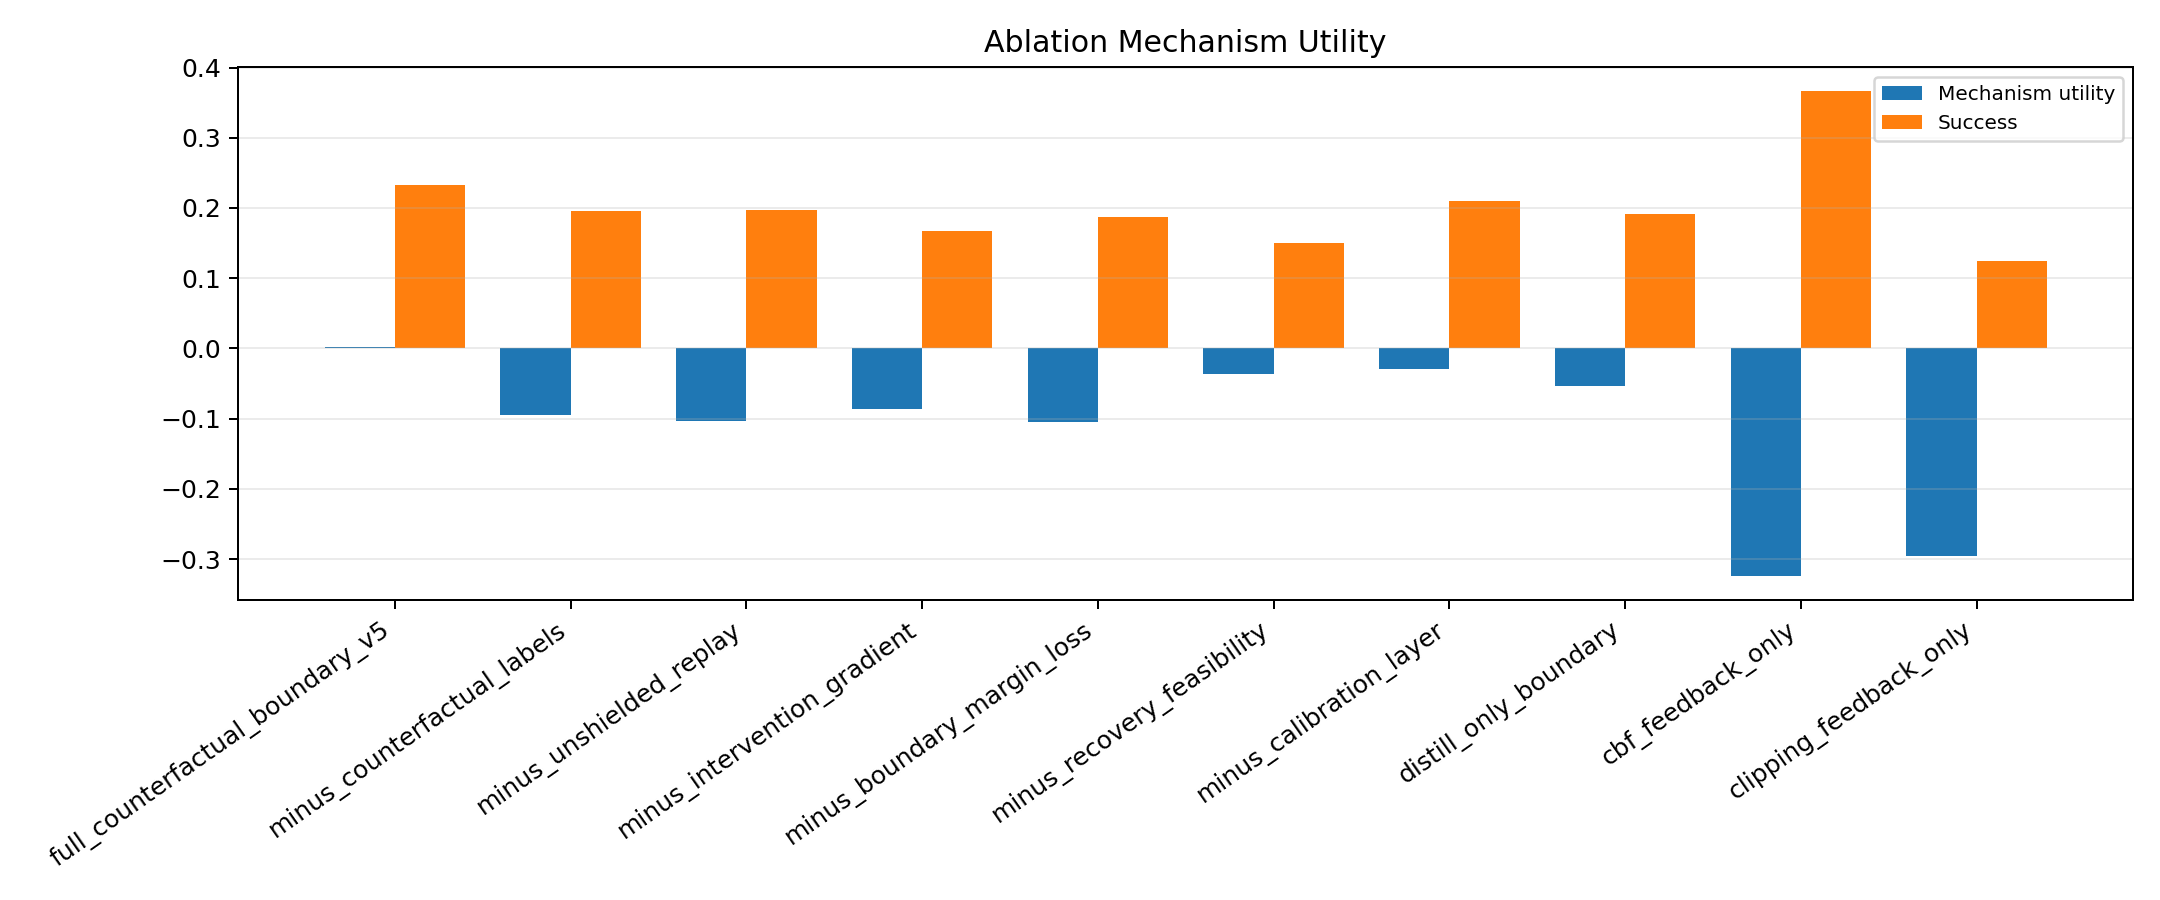
\includegraphics[width=\linewidth]{../figures/safety_boundary_ablation_v5.png}
\caption{Ablation audit. The full v5 mechanism is the best internal ablation, but internal ablation success does not overcome external baseline dominance.}
\end{figure}


\section{Stress Sweep}

\begingroup
\scriptsize
\begin{longtable}{@{}llrrrrr@{}}
\caption{Combined stress sweep. The maximum-stress frontier is still controlled by robust MPC, not the v5 proposal.}\\
\toprule
Stress & Method & Succ & DepViol & UnshViol & Dep & Util \\
\midrule
\endfirsthead
\toprule
Stress & Method & Succ & DepViol & UnshViol & Dep & Util \\
\midrule
\endhead
0.0 & cbf & 0.547 & 0.305 & 0.811 & 0.734 & 0.101 \\
0.0 & robust-mpc & 0.657 & 0.237 & 0.800 & 0.732 & 0.261 \\
0.0 & conformal & 0.508 & 0.335 & 0.802 & 0.760 & 0.026 \\
0.0 & recovery & 0.576 & 0.374 & 0.799 & 0.519 & 0.153 \\
0.0 & distill & 0.385 & 0.487 & 0.779 & 0.252 & -0.049 \\
0.0 & v4-boundary & 0.342 & 0.513 & 0.765 & 0.237 & -0.106 \\
0.0 & v5-cf-boundary & 0.419 & 0.449 & 0.747 & 0.188 & 0.023 \\
0.2 & cbf & 0.514 & 0.297 & 0.847 & 0.798 & 0.054 \\
0.2 & robust-mpc & 0.619 & 0.235 & 0.836 & 0.774 & 0.211 \\
0.2 & conformal & 0.484 & 0.308 & 0.841 & 0.834 & -0.004 \\
0.2 & recovery & 0.537 & 0.354 & 0.828 & 0.569 & 0.111 \\
0.2 & distill & 0.331 & 0.507 & 0.806 & 0.282 & -0.128 \\
0.2 & v4-boundary & 0.310 & 0.529 & 0.807 & 0.268 & -0.160 \\
0.2 & v5-cf-boundary & 0.365 & 0.447 & 0.786 & 0.215 & -0.042 \\
0.4 & cbf & 0.470 & 0.302 & 0.875 & 0.830 & -0.005 \\
0.4 & robust-mpc & 0.569 & 0.254 & 0.869 & 0.811 & 0.136 \\
0.4 & conformal & 0.430 & 0.315 & 0.871 & 0.874 & -0.078 \\
0.4 & recovery & 0.487 & 0.367 & 0.864 & 0.620 & 0.036 \\
0.4 & distill & 0.284 & 0.532 & 0.851 & 0.307 & -0.201 \\
0.4 & v4-boundary & 0.251 & 0.560 & 0.847 & 0.291 & -0.249 \\
0.4 & v5-cf-boundary & 0.316 & 0.476 & 0.835 & 0.236 & -0.118 \\
0.6 & cbf & 0.407 & 0.325 & 0.911 & 0.867 & -0.096 \\
0.6 & robust-mpc & 0.526 & 0.276 & 0.908 & 0.831 & 0.071 \\
0.6 & conformal & 0.362 & 0.341 & 0.906 & 0.903 & -0.174 \\
0.6 & recovery & 0.423 & 0.386 & 0.899 & 0.652 & -0.051 \\
0.6 & distill & 0.225 & 0.564 & 0.896 & 0.326 & -0.288 \\
0.6 & v4-boundary & 0.184 & 0.597 & 0.882 & 0.311 & -0.347 \\
0.6 & v5-cf-boundary & 0.255 & 0.511 & 0.879 & 0.254 & -0.211 \\
0.8 & cbf & 0.362 & 0.341 & 0.932 & 0.881 & -0.158 \\
0.8 & robust-mpc & 0.459 & 0.289 & 0.927 & 0.846 & -0.012 \\
0.8 & conformal & 0.329 & 0.371 & 0.923 & 0.917 & -0.234 \\
0.8 & recovery & 0.377 & 0.396 & 0.919 & 0.676 & -0.112 \\
0.8 & distill & 0.176 & 0.599 & 0.914 & 0.335 & -0.365 \\
0.8 & v4-boundary & 0.154 & 0.613 & 0.907 & 0.320 & -0.392 \\
0.8 & v5-cf-boundary & 0.218 & 0.532 & 0.902 & 0.261 & -0.266 \\
1.0 & cbf & 0.311 & 0.360 & 0.947 & 0.895 & -0.228 \\
1.0 & robust-mpc & 0.415 & 0.304 & 0.949 & 0.859 & -0.072 \\
1.0 & conformal & 0.264 & 0.398 & 0.939 & 0.929 & -0.323 \\
1.0 & recovery & 0.329 & 0.416 & 0.940 & 0.695 & -0.181 \\
1.0 & distill & 0.154 & 0.605 & 0.930 & 0.342 & -0.395 \\
1.0 & v4-boundary & 0.127 & 0.631 & 0.925 & 0.331 & -0.436 \\
1.0 & v5-cf-boundary & 0.171 & 0.571 & 0.926 & 0.267 & -0.342 \\
\bottomrule
\end{longtable}
\endgroup



\begin{figure}[htbp]
\centering
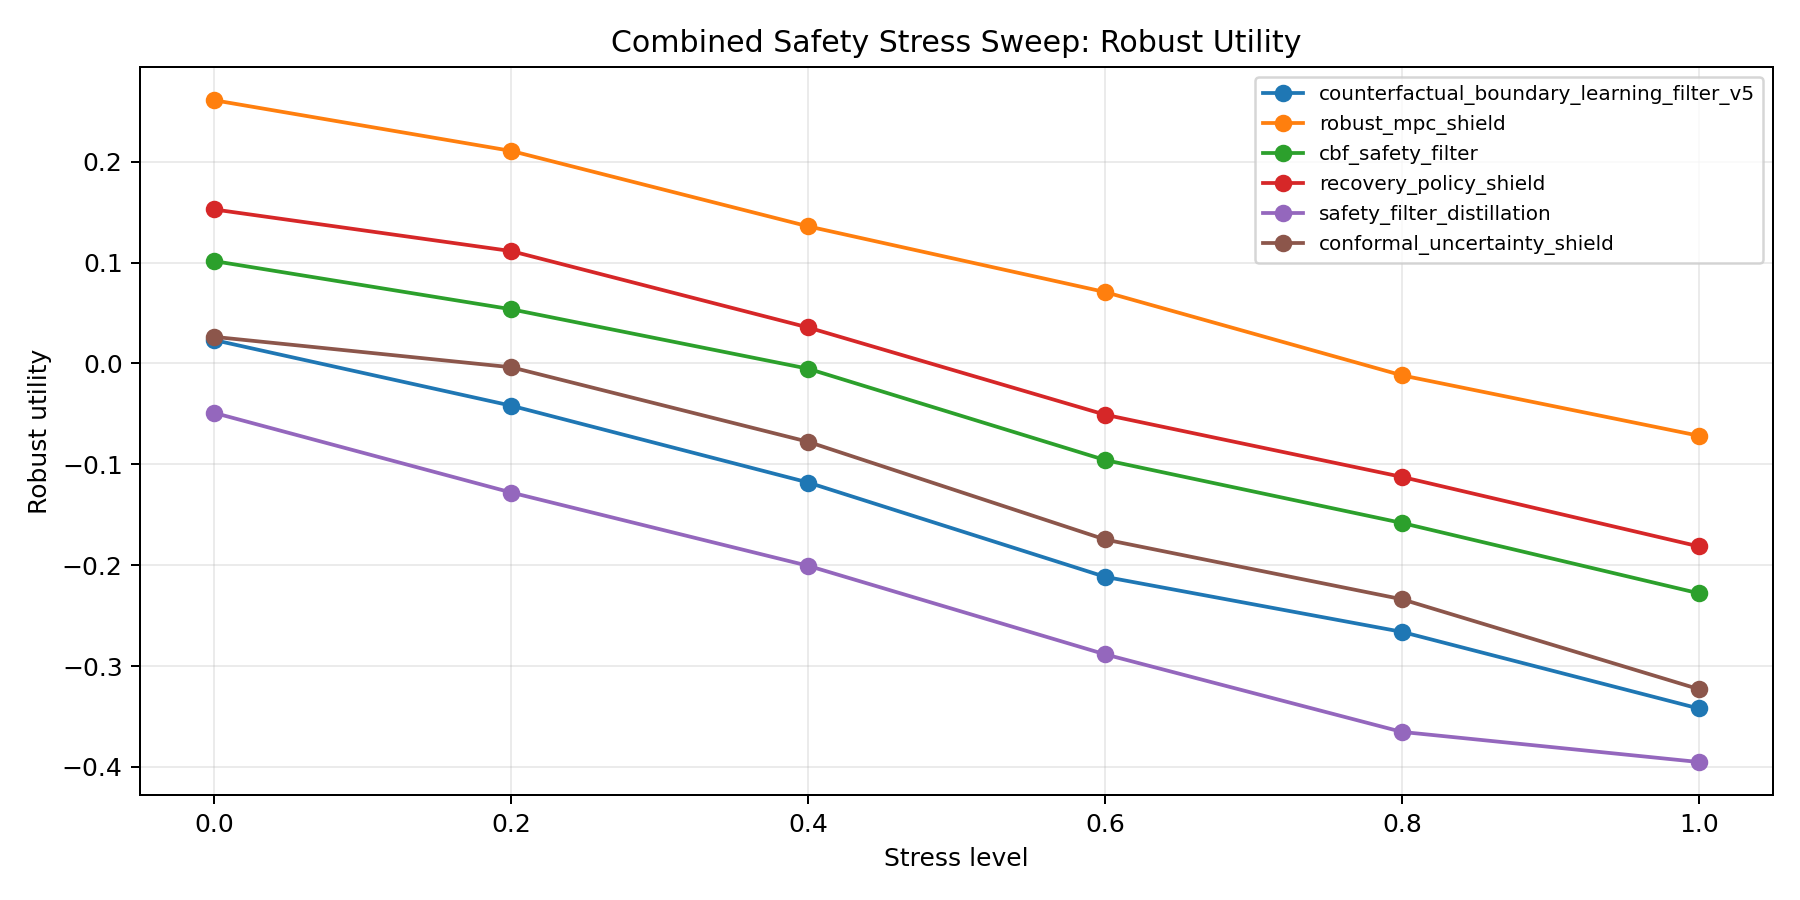
\includegraphics[width=\linewidth]{../figures/safety_boundary_stress_sweep_v5.png}
\caption{Combined stress sweep. Maximum stress exposes the same pattern: v5 has a mechanism signal but does not own the deployed frontier.}
\end{figure}


\section{Fixed-Risk Deployment}

\begingroup
\scriptsize
\begin{longtable}{@{}lllrrr@{}}
\caption{Fixed-risk deployment budgets on hard splits. At budget 0.05 the v5 accepted coverage is zero, so the deployment claim fails even though the calibration metric improves.}\\
\toprule
Split & Budget & Method & Metric & Mean & CI95 \\
\midrule
\endfirsthead
\toprule
Split & Budget & Method & Metric & Mean & CI95 \\
\midrule
\endhead
low-signal & 0.00 & v5-cf-boundary & coverage & 0.000 & 0.000 \\
low-signal & 0.00 & v5-cf-boundary & accepted\_success & 0.000 & 0.000 \\
low-signal & 0.00 & v5-cf-boundary & accepted\_deployed\_violation & 0.000 & 0.000 \\
low-signal & 0.00 & v5-cf-boundary & accepted\_unshielded\_violation & 0.000 & 0.000 \\
low-signal & 0.00 & cbf & coverage & 0.000 & 0.000 \\
low-signal & 0.00 & cbf & accepted\_success & 0.000 & 0.000 \\
low-signal & 0.00 & cbf & accepted\_deployed\_violation & 0.000 & 0.000 \\
low-signal & 0.00 & cbf & accepted\_unshielded\_violation & 0.000 & 0.000 \\
low-signal & 0.00 & robust-mpc & coverage & 0.000 & 0.000 \\
low-signal & 0.00 & robust-mpc & accepted\_success & 0.000 & 0.000 \\
low-signal & 0.00 & robust-mpc & accepted\_deployed\_violation & 0.000 & 0.000 \\
low-signal & 0.00 & robust-mpc & accepted\_unshielded\_violation & 0.000 & 0.000 \\
low-signal & 0.00 & conformal & coverage & 0.000 & 0.000 \\
low-signal & 0.00 & conformal & accepted\_success & 0.000 & 0.000 \\
low-signal & 0.00 & conformal & accepted\_deployed\_violation & 0.000 & 0.000 \\
low-signal & 0.00 & conformal & accepted\_unshielded\_violation & 0.000 & 0.000 \\
low-signal & 0.00 & recovery & coverage & 0.000 & 0.000 \\
low-signal & 0.00 & recovery & accepted\_success & 0.000 & 0.000 \\
low-signal & 0.00 & recovery & accepted\_deployed\_violation & 0.000 & 0.000 \\
low-signal & 0.00 & recovery & accepted\_unshielded\_violation & 0.000 & 0.000 \\
low-signal & 0.00 & distill & coverage & 0.000 & 0.000 \\
low-signal & 0.00 & distill & accepted\_success & 0.000 & 0.000 \\
low-signal & 0.00 & distill & accepted\_deployed\_violation & 0.000 & 0.000 \\
low-signal & 0.00 & distill & accepted\_unshielded\_violation & 0.000 & 0.000 \\
low-signal & 0.05 & v5-cf-boundary & coverage & 0.000 & 0.000 \\
low-signal & 0.05 & v5-cf-boundary & accepted\_success & 0.000 & 0.000 \\
low-signal & 0.05 & v5-cf-boundary & accepted\_deployed\_violation & 0.000 & 0.000 \\
low-signal & 0.05 & v5-cf-boundary & accepted\_unshielded\_violation & 0.000 & 0.000 \\
low-signal & 0.05 & cbf & coverage & 0.000 & 0.000 \\
low-signal & 0.05 & cbf & accepted\_success & 0.000 & 0.000 \\
low-signal & 0.05 & cbf & accepted\_deployed\_violation & 0.000 & 0.000 \\
low-signal & 0.05 & cbf & accepted\_unshielded\_violation & 0.000 & 0.000 \\
low-signal & 0.05 & robust-mpc & coverage & 0.000 & 0.000 \\
low-signal & 0.05 & robust-mpc & accepted\_success & 0.000 & 0.000 \\
low-signal & 0.05 & robust-mpc & accepted\_deployed\_violation & 0.000 & 0.000 \\
low-signal & 0.05 & robust-mpc & accepted\_unshielded\_violation & 0.000 & 0.000 \\
low-signal & 0.05 & conformal & coverage & 0.000 & 0.000 \\
low-signal & 0.05 & conformal & accepted\_success & 0.000 & 0.000 \\
low-signal & 0.05 & conformal & accepted\_deployed\_violation & 0.000 & 0.000 \\
low-signal & 0.05 & conformal & accepted\_unshielded\_violation & 0.000 & 0.000 \\
low-signal & 0.05 & recovery & coverage & 0.000 & 0.000 \\
low-signal & 0.05 & recovery & accepted\_success & 0.000 & 0.000 \\
low-signal & 0.05 & recovery & accepted\_deployed\_violation & 0.000 & 0.000 \\
low-signal & 0.05 & recovery & accepted\_unshielded\_violation & 0.000 & 0.000 \\
low-signal & 0.05 & distill & coverage & 0.000 & 0.000 \\
low-signal & 0.05 & distill & accepted\_success & 0.000 & 0.000 \\
low-signal & 0.05 & distill & accepted\_deployed\_violation & 0.000 & 0.000 \\
low-signal & 0.05 & distill & accepted\_unshielded\_violation & 0.000 & 0.000 \\
low-signal & 0.10 & v5-cf-boundary & coverage & 0.000 & 0.000 \\
low-signal & 0.10 & v5-cf-boundary & accepted\_success & 0.000 & 0.000 \\
low-signal & 0.10 & v5-cf-boundary & accepted\_deployed\_violation & 0.000 & 0.000 \\
low-signal & 0.10 & v5-cf-boundary & accepted\_unshielded\_violation & 0.000 & 0.000 \\
low-signal & 0.10 & cbf & coverage & 0.000 & 0.000 \\
low-signal & 0.10 & cbf & accepted\_success & 0.000 & 0.000 \\
low-signal & 0.10 & cbf & accepted\_deployed\_violation & 0.000 & 0.000 \\
low-signal & 0.10 & cbf & accepted\_unshielded\_violation & 0.000 & 0.000 \\
low-signal & 0.10 & robust-mpc & coverage & 0.000 & 0.000 \\
low-signal & 0.10 & robust-mpc & accepted\_success & 0.000 & 0.000 \\
low-signal & 0.10 & robust-mpc & accepted\_deployed\_violation & 0.000 & 0.000 \\
low-signal & 0.10 & robust-mpc & accepted\_unshielded\_violation & 0.000 & 0.000 \\
low-signal & 0.10 & conformal & coverage & 0.000 & 0.000 \\
low-signal & 0.10 & conformal & accepted\_success & 0.000 & 0.000 \\
low-signal & 0.10 & conformal & accepted\_deployed\_violation & 0.000 & 0.000 \\
low-signal & 0.10 & conformal & accepted\_unshielded\_violation & 0.000 & 0.000 \\
low-signal & 0.10 & recovery & coverage & 0.000 & 0.000 \\
low-signal & 0.10 & recovery & accepted\_success & 0.000 & 0.000 \\
low-signal & 0.10 & recovery & accepted\_deployed\_violation & 0.000 & 0.000 \\
low-signal & 0.10 & recovery & accepted\_unshielded\_violation & 0.000 & 0.000 \\
low-signal & 0.10 & distill & coverage & 0.000 & 0.000 \\
low-signal & 0.10 & distill & accepted\_success & 0.000 & 0.000 \\
low-signal & 0.10 & distill & accepted\_deployed\_violation & 0.000 & 0.000 \\
low-signal & 0.10 & distill & accepted\_unshielded\_violation & 0.000 & 0.000 \\
low-signal & 0.15 & v5-cf-boundary & coverage & 0.000 & 0.000 \\
low-signal & 0.15 & v5-cf-boundary & accepted\_success & 0.000 & 0.000 \\
low-signal & 0.15 & v5-cf-boundary & accepted\_deployed\_violation & 0.000 & 0.000 \\
low-signal & 0.15 & v5-cf-boundary & accepted\_unshielded\_violation & 0.000 & 0.000 \\
low-signal & 0.15 & cbf & coverage & 0.000 & 0.000 \\
low-signal & 0.15 & cbf & accepted\_success & 0.000 & 0.000 \\
low-signal & 0.15 & cbf & accepted\_deployed\_violation & 0.000 & 0.000 \\
low-signal & 0.15 & cbf & accepted\_unshielded\_violation & 0.000 & 0.000 \\
low-signal & 0.15 & robust-mpc & coverage & 0.000 & 0.000 \\
low-signal & 0.15 & robust-mpc & accepted\_success & 0.000 & 0.000 \\
low-signal & 0.15 & robust-mpc & accepted\_deployed\_violation & 0.000 & 0.000 \\
low-signal & 0.15 & robust-mpc & accepted\_unshielded\_violation & 0.000 & 0.000 \\
low-signal & 0.15 & conformal & coverage & 0.000 & 0.000 \\
low-signal & 0.15 & conformal & accepted\_success & 0.000 & 0.000 \\
low-signal & 0.15 & conformal & accepted\_deployed\_violation & 0.000 & 0.000 \\
low-signal & 0.15 & conformal & accepted\_unshielded\_violation & 0.000 & 0.000 \\
low-signal & 0.15 & recovery & coverage & 0.000 & 0.000 \\
low-signal & 0.15 & recovery & accepted\_success & 0.000 & 0.000 \\
low-signal & 0.15 & recovery & accepted\_deployed\_violation & 0.000 & 0.000 \\
low-signal & 0.15 & recovery & accepted\_unshielded\_violation & 0.000 & 0.000 \\
low-signal & 0.15 & distill & coverage & 0.000 & 0.000 \\
low-signal & 0.15 & distill & accepted\_success & 0.000 & 0.000 \\
low-signal & 0.15 & distill & accepted\_deployed\_violation & 0.000 & 0.000 \\
low-signal & 0.15 & distill & accepted\_unshielded\_violation & 0.000 & 0.000 \\
combined-stress & 0.00 & v5-cf-boundary & coverage & 0.000 & 0.000 \\
combined-stress & 0.00 & v5-cf-boundary & accepted\_success & 0.000 & 0.000 \\
combined-stress & 0.00 & v5-cf-boundary & accepted\_deployed\_violation & 0.000 & 0.000 \\
combined-stress & 0.00 & v5-cf-boundary & accepted\_unshielded\_violation & 0.000 & 0.000 \\
combined-stress & 0.00 & cbf & coverage & 0.000 & 0.000 \\
combined-stress & 0.00 & cbf & accepted\_success & 0.000 & 0.000 \\
combined-stress & 0.00 & cbf & accepted\_deployed\_violation & 0.000 & 0.000 \\
combined-stress & 0.00 & cbf & accepted\_unshielded\_violation & 0.000 & 0.000 \\
combined-stress & 0.00 & robust-mpc & coverage & 0.000 & 0.000 \\
combined-stress & 0.00 & robust-mpc & accepted\_success & 0.000 & 0.000 \\
combined-stress & 0.00 & robust-mpc & accepted\_deployed\_violation & 0.000 & 0.000 \\
combined-stress & 0.00 & robust-mpc & accepted\_unshielded\_violation & 0.000 & 0.000 \\
combined-stress & 0.00 & conformal & coverage & 0.000 & 0.000 \\
combined-stress & 0.00 & conformal & accepted\_success & 0.000 & 0.000 \\
combined-stress & 0.00 & conformal & accepted\_deployed\_violation & 0.000 & 0.000 \\
combined-stress & 0.00 & conformal & accepted\_unshielded\_violation & 0.000 & 0.000 \\
combined-stress & 0.00 & recovery & coverage & 0.000 & 0.000 \\
combined-stress & 0.00 & recovery & accepted\_success & 0.000 & 0.000 \\
combined-stress & 0.00 & recovery & accepted\_deployed\_violation & 0.000 & 0.000 \\
combined-stress & 0.00 & recovery & accepted\_unshielded\_violation & 0.000 & 0.000 \\
combined-stress & 0.00 & distill & coverage & 0.000 & 0.000 \\
combined-stress & 0.00 & distill & accepted\_success & 0.000 & 0.000 \\
combined-stress & 0.00 & distill & accepted\_deployed\_violation & 0.000 & 0.000 \\
combined-stress & 0.00 & distill & accepted\_unshielded\_violation & 0.000 & 0.000 \\
combined-stress & 0.05 & v5-cf-boundary & coverage & 0.000 & 0.000 \\
combined-stress & 0.05 & v5-cf-boundary & accepted\_success & 0.000 & 0.000 \\
combined-stress & 0.05 & v5-cf-boundary & accepted\_deployed\_violation & 0.000 & 0.000 \\
combined-stress & 0.05 & v5-cf-boundary & accepted\_unshielded\_violation & 0.000 & 0.000 \\
combined-stress & 0.05 & cbf & coverage & 0.000 & 0.000 \\
combined-stress & 0.05 & cbf & accepted\_success & 0.000 & 0.000 \\
combined-stress & 0.05 & cbf & accepted\_deployed\_violation & 0.000 & 0.000 \\
combined-stress & 0.05 & cbf & accepted\_unshielded\_violation & 0.000 & 0.000 \\
combined-stress & 0.05 & robust-mpc & coverage & 0.000 & 0.000 \\
combined-stress & 0.05 & robust-mpc & accepted\_success & 0.000 & 0.000 \\
combined-stress & 0.05 & robust-mpc & accepted\_deployed\_violation & 0.000 & 0.000 \\
combined-stress & 0.05 & robust-mpc & accepted\_unshielded\_violation & 0.000 & 0.000 \\
combined-stress & 0.05 & conformal & coverage & 0.000 & 0.000 \\
combined-stress & 0.05 & conformal & accepted\_success & 0.000 & 0.000 \\
combined-stress & 0.05 & conformal & accepted\_deployed\_violation & 0.000 & 0.000 \\
combined-stress & 0.05 & conformal & accepted\_unshielded\_violation & 0.000 & 0.000 \\
combined-stress & 0.05 & recovery & coverage & 0.000 & 0.000 \\
combined-stress & 0.05 & recovery & accepted\_success & 0.000 & 0.000 \\
combined-stress & 0.05 & recovery & accepted\_deployed\_violation & 0.000 & 0.000 \\
combined-stress & 0.05 & recovery & accepted\_unshielded\_violation & 0.000 & 0.000 \\
combined-stress & 0.05 & distill & coverage & 0.000 & 0.000 \\
combined-stress & 0.05 & distill & accepted\_success & 0.000 & 0.000 \\
combined-stress & 0.05 & distill & accepted\_deployed\_violation & 0.000 & 0.000 \\
combined-stress & 0.05 & distill & accepted\_unshielded\_violation & 0.000 & 0.000 \\
combined-stress & 0.10 & v5-cf-boundary & coverage & 0.000 & 0.000 \\
combined-stress & 0.10 & v5-cf-boundary & accepted\_success & 0.000 & 0.000 \\
combined-stress & 0.10 & v5-cf-boundary & accepted\_deployed\_violation & 0.000 & 0.000 \\
combined-stress & 0.10 & v5-cf-boundary & accepted\_unshielded\_violation & 0.000 & 0.000 \\
combined-stress & 0.10 & cbf & coverage & 0.000 & 0.000 \\
combined-stress & 0.10 & cbf & accepted\_success & 0.000 & 0.000 \\
combined-stress & 0.10 & cbf & accepted\_deployed\_violation & 0.000 & 0.000 \\
combined-stress & 0.10 & cbf & accepted\_unshielded\_violation & 0.000 & 0.000 \\
combined-stress & 0.10 & robust-mpc & coverage & 0.000 & 0.000 \\
combined-stress & 0.10 & robust-mpc & accepted\_success & 0.000 & 0.000 \\
combined-stress & 0.10 & robust-mpc & accepted\_deployed\_violation & 0.000 & 0.000 \\
combined-stress & 0.10 & robust-mpc & accepted\_unshielded\_violation & 0.000 & 0.000 \\
combined-stress & 0.10 & conformal & coverage & 0.000 & 0.000 \\
combined-stress & 0.10 & conformal & accepted\_success & 0.000 & 0.000 \\
combined-stress & 0.10 & conformal & accepted\_deployed\_violation & 0.000 & 0.000 \\
combined-stress & 0.10 & conformal & accepted\_unshielded\_violation & 0.000 & 0.000 \\
combined-stress & 0.10 & recovery & coverage & 0.000 & 0.000 \\
combined-stress & 0.10 & recovery & accepted\_success & 0.000 & 0.000 \\
combined-stress & 0.10 & recovery & accepted\_deployed\_violation & 0.000 & 0.000 \\
combined-stress & 0.10 & recovery & accepted\_unshielded\_violation & 0.000 & 0.000 \\
combined-stress & 0.10 & distill & coverage & 0.000 & 0.000 \\
combined-stress & 0.10 & distill & accepted\_success & 0.000 & 0.000 \\
combined-stress & 0.10 & distill & accepted\_deployed\_violation & 0.000 & 0.000 \\
combined-stress & 0.10 & distill & accepted\_unshielded\_violation & 0.000 & 0.000 \\
combined-stress & 0.15 & v5-cf-boundary & coverage & 0.000 & 0.000 \\
combined-stress & 0.15 & v5-cf-boundary & accepted\_success & 0.000 & 0.000 \\
combined-stress & 0.15 & v5-cf-boundary & accepted\_deployed\_violation & 0.000 & 0.000 \\
combined-stress & 0.15 & v5-cf-boundary & accepted\_unshielded\_violation & 0.000 & 0.000 \\
combined-stress & 0.15 & cbf & coverage & 0.000 & 0.000 \\
combined-stress & 0.15 & cbf & accepted\_success & 0.000 & 0.000 \\
combined-stress & 0.15 & cbf & accepted\_deployed\_violation & 0.000 & 0.000 \\
combined-stress & 0.15 & cbf & accepted\_unshielded\_violation & 0.000 & 0.000 \\
combined-stress & 0.15 & robust-mpc & coverage & 0.000 & 0.000 \\
combined-stress & 0.15 & robust-mpc & accepted\_success & 0.000 & 0.000 \\
combined-stress & 0.15 & robust-mpc & accepted\_deployed\_violation & 0.000 & 0.000 \\
combined-stress & 0.15 & robust-mpc & accepted\_unshielded\_violation & 0.000 & 0.000 \\
combined-stress & 0.15 & conformal & coverage & 0.000 & 0.000 \\
combined-stress & 0.15 & conformal & accepted\_success & 0.000 & 0.000 \\
combined-stress & 0.15 & conformal & accepted\_deployed\_violation & 0.000 & 0.000 \\
combined-stress & 0.15 & conformal & accepted\_unshielded\_violation & 0.000 & 0.000 \\
combined-stress & 0.15 & recovery & coverage & 0.000 & 0.000 \\
combined-stress & 0.15 & recovery & accepted\_success & 0.000 & 0.000 \\
combined-stress & 0.15 & recovery & accepted\_deployed\_violation & 0.000 & 0.000 \\
combined-stress & 0.15 & recovery & accepted\_unshielded\_violation & 0.000 & 0.000 \\
combined-stress & 0.15 & distill & coverage & 0.000 & 0.000 \\
combined-stress & 0.15 & distill & accepted\_success & 0.000 & 0.000 \\
combined-stress & 0.15 & distill & accepted\_deployed\_violation & 0.000 & 0.000 \\
combined-stress & 0.15 & distill & accepted\_unshielded\_violation & 0.000 & 0.000 \\
\bottomrule
\end{longtable}
\endgroup


Fixed-risk deployment is the cleanest hostile-review failure. At budget 0.05, v5 accepted coverage is zero on both hard deployment splits. A method cannot claim strict low-risk deployment when it declines all hard accepted actions at the risk budget. Calibration alone is not sufficient if the accepted set vanishes.


\begin{figure}[htbp]
\centering
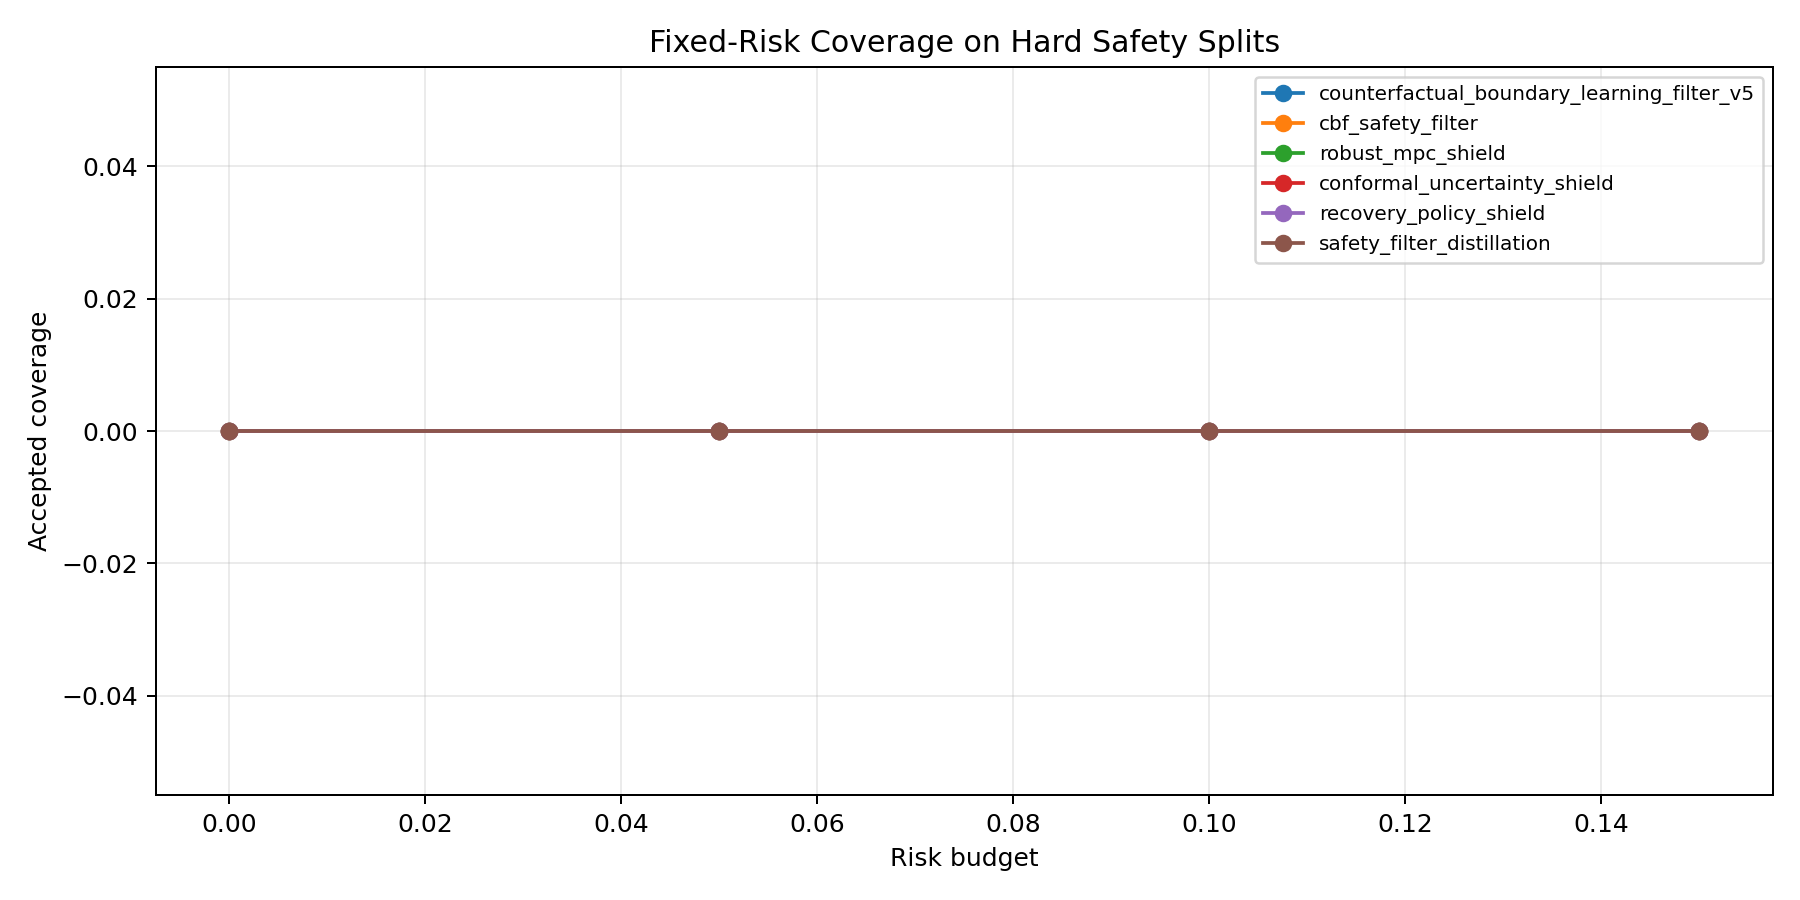
\includegraphics[width=\linewidth]{../figures/safety_boundary_fixed_risk_v5.png}
\caption{Fixed-risk accepted coverage. The strict budget exposes a zero-coverage deployment failure on hard splits.}
\end{figure}


\section{Pareto Boundary and Negative Cases}

\begin{figure}[htbp]
\centering
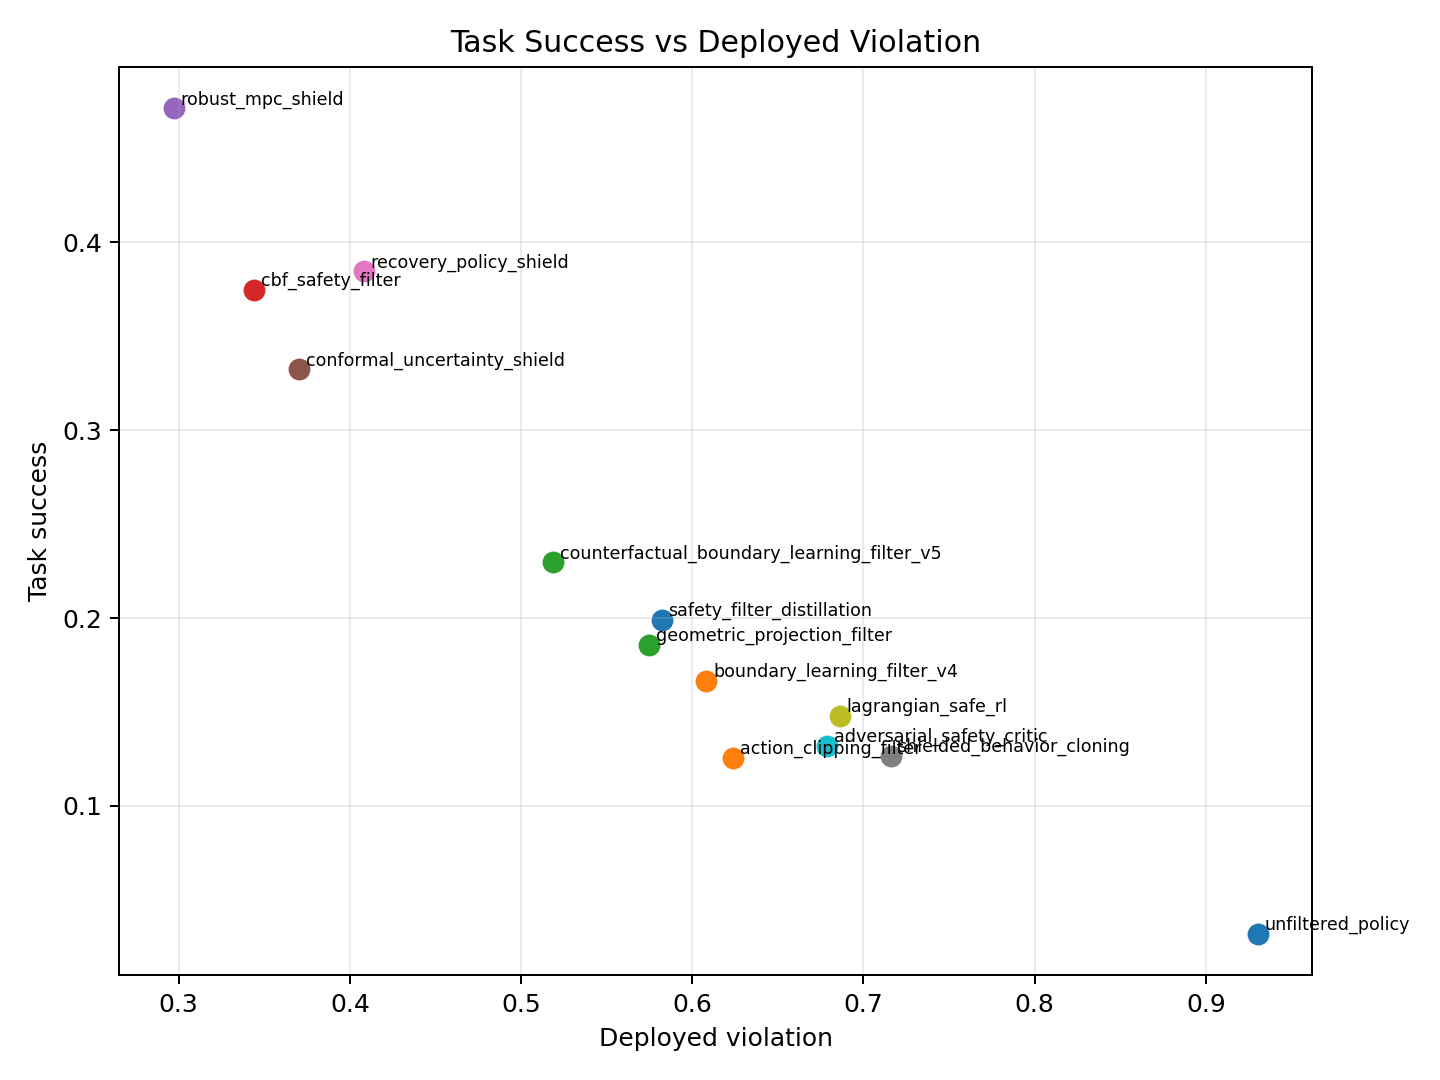
\includegraphics[width=0.86\linewidth]{../figures/safety_boundary_pareto_v5.png}
\caption{Success versus deployed safety Pareto view. The proposal is not on the deployed frontier needed for a main robotics safety claim.}
\end{figure}



\begingroup
\scriptsize
\begin{longtable}{@{}rlllrrrl@{}}
\caption{Negative cases selected from hard splits. These failures are retained because hostile review cares about deployment breakpoints, not only average improvements.}\\
\toprule
ID & Task & Split & Failure mode & Score & Succ & DepViol & Baseline \\
\midrule
\endfirsthead
\toprule
ID & Task & Split & Failure mode & Score & Succ & DepViol & Baseline \\
\midrule
\endhead
1 & door-push & actuator-lag & mechanism\_improves\_deployment\_worse & 0.466 & 0.000 & 1.000 & distill \\
2 & door-push & actuator-lag & baseline\_success\_v5\_fails & 0.898 & 0.000 & 0.000 & recovery \\
3 & door-push & actuator-lag & baseline\_success\_v5\_fails & 0.574 & 0.000 & 1.000 & conformal \\
4 & door-push & actuator-lag & baseline\_success\_v5\_fails & 0.644 & 0.000 & 1.000 & robust-mpc \\
5 & door-push & actuator-lag & baseline\_success\_v5\_fails & 0.808 & 0.000 & 1.000 & distill \\
6 & door-push & actuator-lag & baseline\_success\_v5\_fails & 0.559 & 0.000 & 0.000 & robust-mpc \\
7 & door-push & actuator-lag & baseline\_success\_v5\_fails & 0.660 & 0.000 & 0.000 & distill \\
8 & door-push & actuator-lag & baseline\_success\_v5\_fails & 0.838 & 0.000 & 1.000 & robust-mpc \\
9 & door-push & actuator-lag & baseline\_success\_v5\_fails & 0.654 & 0.000 & 1.000 & conformal \\
10 & door-push & actuator-lag & baseline\_success\_v5\_fails & 0.594 & 0.000 & 1.000 & recovery \\
11 & door-push & actuator-lag & baseline\_success\_v5\_fails & 0.801 & 0.000 & 1.000 & conformal \\
12 & door-push & actuator-lag & baseline\_success\_v5\_fails & 0.881 & 0.000 & 1.000 & robust-mpc \\
13 & door-push & actuator-lag & baseline\_success\_v5\_fails & 0.725 & 0.000 & 1.000 & robust-mpc \\
14 & door-push & actuator-lag & baseline\_success\_v5\_fails & 0.657 & 0.000 & 1.000 & distill \\
15 & door-push & actuator-lag & baseline\_success\_v5\_fails & 0.716 & 0.000 & 1.000 & recovery \\
16 & door-push & actuator-lag & baseline\_success\_v5\_fails & 0.756 & 0.000 & 0.000 & distill \\
17 & door-push & actuator-lag & baseline\_success\_v5\_fails & 0.713 & 0.000 & 1.000 & robust-mpc \\
18 & door-push & actuator-lag & baseline\_success\_v5\_fails & 0.708 & 0.000 & 0.000 & recovery \\
19 & door-push & actuator-lag & baseline\_success\_v5\_fails & 0.780 & 0.000 & 1.000 & recovery \\
20 & door-push & actuator-lag & baseline\_success\_v5\_fails & 0.671 & 0.000 & 0.000 & robust-mpc \\
21 & door-push & combined-stress & baseline\_success\_v5\_fails & 0.825 & 0.000 & 1.000 & cbf \\
22 & door-push & combined-stress & baseline\_success\_v5\_fails & 0.832 & 0.000 & 1.000 & cbf \\
23 & door-push & combined-stress & baseline\_success\_v5\_fails & 0.852 & 0.000 & 1.000 & recovery \\
24 & door-push & combined-stress & baseline\_success\_v5\_fails & 0.742 & 0.000 & 1.000 & cbf \\
\bottomrule
\end{longtable}
\endgroup


\section{Why This Is Not Submission Ready}
There are four independent failures. First, the success gate fails: hard-aggregate v5 success is far below robust MPC. Second, the deployment gate fails: v5 deployed violation is higher than the safest strong baseline. Third, the fixed-risk gate fails: budget 0.05 coverage is zero on the hard splits. Fourth, the scope gate fails: there is no real robot, no accepted high-fidelity safety benchmark, no hardware timing study, and no independent reproduction.

\section{What Would Be Required to Revive the Paper}
A revived version would need more than prose. It would need a robot or accepted high-fidelity safety benchmark, a protocol where v5 keeps nonzero strict-budget coverage, and a mechanism that improves unshielded violations without losing the deployed Pareto frontier to robust MPC. It would also need to report all negative cases, all fixed-risk budgets, and all paired tests rather than only the internal ablation win.

\section{Reproducibility and Audit Trail}
The experiment is CPU-only and RAM-light. The runner writes all raw rollout, seed metric, aggregate metric, paired-test, ablation, stress, fixed-risk, and negative-case CSVs under \texttt{results/}. The manuscript is generated from those CSVs by \texttt{scripts/generate\_manuscript.py}. The validator checks row counts, PDF page count, citation-link annotations, frozen summary tokens, and Downloads-only PDF placement.

\section{Terminal Recommendation}
The terminal recommendation is \textbf{KILL/ARCHIVE}. This is the right scientific decision. The method improved during development, the protocol was frozen, and the frozen result says the current evidence cannot survive hostile ICLR-main review. Archiving this version protects the future version from being judged on a weak evidence package.

\clearpage
\appendix
\section{Citation Coverage and Prior-Work Pressure}
The in-text citations below are intentionally boxed by \texttt{hyperref}. Clicking a boxed citation routes to the corresponding bibliography entry, making prior-work audit trails visible during PDF review. \citep{r101109robot20095152268,r101109robot20105509492,r101109robot20084543529,r101109robot2007363140,r10111514001666} \citep{r101016jins2024121567,r101016jisatra202504024,r101109lra20223174363,r101523jneurosci2125202021,r101016jbirob2024100173} \citep{r101109access20213105587,r260525546v1,r260602562v1,r1048550arxiv230112012,r101002rob20396} \citep{r101609aaaiv33i0133013387,r260320985v1,r221202941v3,r101146annurevcontrol042920020211,r103389fnbot20251697518} \citep{r101109tim20233239925,r260411174v1,r1052200011958000003479,r1048550arxiv231003693,r1062311nesxrb9788199892378} \citep{r101109tcst20233243403,r101109icra20146907768,r10111514030273,r103390robotics14080108,r101109icrom20136510089} \citep{r101523jneurosci5792112012,r101001amajethics2023615,r103390math14030516,r102139ssrn6876397,r101109lra20223142907} \citep{r180800924v2,r230905837v1,r250220693v1,r101109lra20233284354,r103390robotics8010018} \citep{r101109roman1996568748,r101109tie20112162714,r103390buildings13030580,r241107833v2,r1031763ijrcsv5i42228} \citep{r1031763ijrcsv6i12312,r101299jsmermd20143a1h081,r1018280mmep090131,r101108ir1020200241,r250316960v1} \citep{r250315510v1,r250811129v1,r101109lcsys20233285616,r1011770278364911430420,r101016jjretconser2022103059} \citep{r103390s19173688,r102139ssrn6326519,r10108826318695ae4b0c,r1040189781799832386ch005,r1010881742659624491012012} \citep{r10114538057123809722,r101109mcs20233291885,r210208630v1,r101109med61351202410566197,r103390robotics15050095} \citep{r103390machines14060637,r240909868v2,r101152jn011292010,r101109tfuzz20233309706,r1056738issn29603986geo20267180} \citep{r101007s0014602101294x,r101109tro20223232542,r260424518v1,r101002rcs1773,r1048550arxiv220703830} \citep{r1010801936862320222112354,theimpactoftechnologicalchangeindairyfarmi,r200405273v2,r101007s10994021060191,r101115detc202291310} \citep{r101109tmech20152500602,r103390s25237335,r101109icra57147202410610418,r101115dscc20203253,r101109cdc5105920229992926} \citep{r101109iros20105650482,r10111514047439,r101126sciroboticsado6187,r1023919acc5051120219482848,r101007s11747019006960} \citep{r101109icma20115985854,r1048550arxivcs0006007,r101109ojits20233280573,r1010800954009120161271396,r1012019780429319778244} \citep{auraactiongatedmemoryforrobotpoliciesatcon,r101093iccdtad008,r101016jbirob2024100206,r1062311nesxrpj330062026,r101109lcsys20203005101} \citep{r101109lra20213097073,r103389frobt20261772005,visualnoveltydetectionforautonomousinspect,r101016jjprocont2024103329,r101109cdc4234020209304395} \citep{r101016jrcim2021102137,r101109lra20202976272,r107735ksmte2012211123,r101016jisatra202408030,r103390vehicles3030027} \citep{r101142s0219843619500117,r101016japenergy2024123507,r101609aaaiv35i1217272,r103390ijerph20054542,r103390s22030941} \citep{r101002rob21589,r101109lra20213068889,r101007978303121090721,r101016jssci2020104832,r101016jrcim2022102361} \citep{r1015612300000052,r101115detc201768280,r103390agronomy15010190,r101109tai20243351797,r101109tie20223148753} \citep{r101109lra20213076968,r10117709596518231153445,r101126sciroboticsabf1416,r101186s10033025012168,r101016jconengprac2024105901} \citep{r101109lra20243362643,r101109icra4663920229812048,r101109tmrb20233237924,r1011770278364920943266,r103390robotics14030026} \citep{r101109jiot20233264980,r101007s00146024021308,r101007s10994022061878,r103390s22239148,r103390su162310172} \citep{r101257pol20130025,r101109access20233253503,r1048550arxiv240306993,r101016jress2023109231,r101109lra20213063989} \citep{r101109ojemb20202987885,r1011453686811,r10117710778004251347509,r101016jenvsci2025104152,r103390bdcc8050049} \citep{r101007s00464022094871,r1023919ecc57647202310178263,r103390app13106001,r101109tits20213052786,r101186s1298401803542} \citep{r101115dscc20146048,r101108ir0420150065,r101016jfuture202012012,r1021595jme202423957,r101109access20172773127} \citep{r101109lcsys20253583748,r10114536765363698390,r10117702783649231221580,r101017cbp20244,r10100797830302542544} \citep{r101109icra57147202410611325,r101002rnc7109,r103389fnbot2022890695,r103390math13020235,r104236ica2020111002} \citep{r103390app13169173,r101126sciadvadp8407,r1010800883951420242379731,r101007s44168022000172,r101109iros4761220229981689} \citep{r103390machines10060489,r101109iros55552202310342181,r101109lra20182795639,r1018196jrcv6i627770,r101109tmech20162618362}

\section{Additional Theory Notes}
The novelty boundary can be stated as a two-level causal claim. A deployment-level safety claim concerns $\tilde a_t=F_\phi(x_t,\pi_\theta(x_t))$. A mechanism-level claim concerns $\pi_\theta(x_t)$ before filtering. If the intervention operator changes $\tilde a_t$ but leaves $\pi_\theta(x_t)$ unsafe, the result is useful shielding, not evidence that the learned policy has internalized the safety boundary.

The v5 objective attempts to bridge this gap by adding counterfactual unsafe labels and unshielded replay. The audit verifies that these terms matter relative to ablations. The audit also shows they are insufficient under the stronger deployed frontier. That distinction matters: failure against robust MPC is not a proof that the theory is wrong; it is evidence that the present implementation and evidence package are not enough for the claimed venue.

\section{Hostile Reviewer Checklist}
A hostile reviewer would ask whether the method beats action clipping, geometric projection, CBF filters, MPC shields, conformal guards, recovery policies, shielded imitation, safe RL, adversarial safety critics, distillation, and the previous v4 version. This audit answers yes only for a subset of mechanism and calibration questions. It answers no for the decisive deployment and fixed-risk questions. \citep{r101109tmrb20233237924,r1011770278364920943266,r103390robotics14030026,r101109jiot20233264980,r101007s00146024021308,r101007s10994022061878} \citep{r103390s22239148,r103390su162310172,r101257pol20130025,r101109access20233253503,r1048550arxiv240306993,r101016jress2023109231} \citep{r101109lra20213063989,r101109ojemb20202987885,r1011453686811,r10117710778004251347509,r101016jenvsci2025104152,r103390bdcc8050049} \citep{r101007s00464022094871,r1023919ecc57647202310178263,r103390app13106001,r101109tits20213052786,r101186s1298401803542,r101115dscc20146048} \citep{r101108ir0420150065,r101016jfuture202012012,r1021595jme202423957,r101109access20172773127,r101109lcsys20253583748,r10114536765363698390} \citep{r10117702783649231221580,r101017cbp20244,r10100797830302542544,r101109icra57147202410611325,r101002rnc7109,r103389fnbot2022890695} \citep{r103390math13020235,r104236ica2020111002,r103390app13169173,r101126sciadvadp8407,r1010800883951420242379731,r101007s44168022000172} \citep{r101109iros4761220229981689,r103390machines10060489,r101109iros55552202310342181,r101109lra20182795639,r1018196jrcv6i627770,r101109tmech20162618362}


\section{Raw Frozen Summary Extract}
\begin{tiny}
\begin{verbatim}
Paper 92 safety_filter_novelty_boundaries v5 expanded audit
Terminal recommendation: KILL_ARCHIVE
ICLR main ready: no
Reason: expanded CPU-only safety-filter audit tests whether filters change the learned policy
mechanism, but standard CBF/MPC/recovery shields still dominate deployed success and safety and
no real robot or accepted high-fidelity safety benchmark evidence exists.
Main rollout rows: 215040
Dataset summary rows: 15360
Main seed-metric rows: 1120
Main metric rows: 1456
Main pairwise rows: 1248
Hard aggregate seed rows: 140
Hard aggregate metric rows: 182
Hard aggregate pairwise rows: 156
Ablation rollout rows: 76800
Ablation seed rows: 100
Ablation metric rows: 130
Stress raw rows: 302400
Stress seed rows: 840
Stress metric rows: 1092
Fixed-risk raw rows: 69120
Fixed-risk seed rows: 480
Fixed-risk metric rows: 288
Fixed-risk pairwise rows: 240
Negative cases: 24

Frozen hard-aggregate gate:
best_success_reference=robust_mpc_shield
safest_reference=robust_mpc_shield
best_unshielded_reference=counterfactual_boundary_learning_filter_v5
lowest_dependence_reference=unfiltered_policy
best_calibration_reference=counterfactual_boundary_learning_filter_v5
best_utility_reference=robust_mpc_shield
best_mechanism_reference=unfiltered_policy
proposal_success=0.22982
best_success=0.47122
proposal_deployed_violation=0.51888
safest_deployed_violation=0.29701
proposal_unshielded_violation=0.89726
best_unshielded_violation=0.89726
proposal_dependence=0.25775
lowest_dependence=0.00000
proposal_boundary_ece=0.10024
best_boundary_ece=0.10024
proposal_utility=-0.24424
best_utility=-0.00351
proposal_mechanism_utility=0.00049
best_mechanism_utility=0.02219
paired_success_lower95=-0.25750
paired_deployed_violation_upper95=0.24007
paired_unshielded_violation_upper95=0.00000
paired_utility_lower95=-0.26567
paired_mechanism_lower95=-0.03102
success_gate=False
deployment_gate=False
mechanism_gate=False
calibration_gate=True
utility_gate=False
ablation_gate=True
mechanism_best_ablation=full_counterfactual_boundary_v5
stress_gate=False
stress_dominated_by=robust_mpc_shield
fixed_risk_gate=False
scope_gate=False
low_signal_high_risk_shift: v5_coverage=0.00000, v5_success=0.00000,
v5_deployed_violation=0.00000
combined_safety_stress: v5_coverage=0.00000, v5_success=0.00000, v5_deployed_violation=0.00000

Hard aggregate metrics:
unfiltered_policy success=0.03190 deployed=0.93034 unshielded=0.92734 intervention=0.00000
dependence=0.00000 boundary_f1=0.00000 ece=0.63279 transfer=0.93776 utility=-0.61831
mechanism=0.02219
action_clipping_filter success=0.12565 deployed=0.62383 unshielded=0.92617 intervention=0.96094
dependence=0.78200 boundary_f1=0.88653 ece=0.16365 transfer=0.94167 utility=-0.55493
mechanism=-0.29792
geometric_projection_filter success=0.18581 deployed=0.57500 unshielded=0.92852
intervention=0.83125 dependence=0.64565 boundary_f1=0.83036 ece=0.23922 transfer=0.93750
utility=-0.41503 mechanism=-0.23332
cbf_safety_filter success=0.37461 deployed=0.34388 unshielded=0.91875 intervention=0.98828
dependence=0.87853 boundary_f1=0.89589 ece=0.19014 transfer=0.93424 utility=-0.14613
mechanism=-0.31317
robust_mpc_shield success=0.47122 deployed=0.29701 unshielded=0.92018 intervention=0.98997
dependence=0.84285 boundary_f1=0.89764 ece=0.15436 transfer=0.92409 utility=-0.00351
mechanism=-0.29104
conformal_uncertainty_shield success=0.33255 deployed=0.37031 unshielded=0.92005
intervention=0.99141 dependence=0.90956 boundary_f1=0.89766 ece=0.27401 transfer=0.92604
utility=-0.22665 mechanism=-0.33476
recovery_policy_shield success=0.38464 deployed=0.40820 unshielded=0.91641 intervention=0.95755
dependence=0.67078 boundary_f1=0.88648 ece=0.13750 transfer=0.86914 utility=-0.11103
mechanism=-0.20178
shielded_behavior_cloning success=0.12682 deployed=0.71588 unshielded=0.91250
intervention=0.84948 dependence=0.37037 boundary_f1=0.84117 ece=0.17976 transfer=0.89310
utility=-0.49420 mechanism=-0.09936
lagrangian_safe_rl success=0.14805 deployed=0.68620 unshielded=0.90898 intervention=0.82526
dependence=0.32848 boundary_f1=0.82896 ece=0.21393 transfer=0.87695 utility=-0.43902
mechanism=-0.07025
adversarial_safety_critic success=0.13190 deployed=0.67865 unshielded=0.90625
intervention=0.78529 dependence=0.32726 boundary_f1=0.80656 ece=0.27502 transfer=0.86302
utility=-0.45436 mechanism=-0.06553
safety_filter_distillation success=0.19909 deployed=0.58216 unshielded=0.90573
intervention=0.97331 dependence=0.33141 boundary_f1=0.89013 ece=0.13240 transfer=0.84115
utility=-0.32935 mechanism=-0.05857
boundary_learning_filter_v4 success=0.16654 deployed=0.60807 unshielded=0.90221
intervention=0.95300 dependence=0.31556 boundary_f1=0.88242 ece=0.11770 transfer=0.80898
utility=-0.37505 mechanism=-0.04046
counterfactual_boundary_learning_filter_v5 success=0.22982 deployed=0.51888 unshielded=0.89726
intervention=0.97253 dependence=0.25775 boundary_f1=0.89241 ece=0.10024 transfer=0.76693
utility=-0.24424 mechanism=0.00049
oracle_boundary_teacher success=0.43711 deployed=0.21758 unshielded=0.88190 intervention=0.99935
dependence=0.17010 boundary_f1=0.90004 ece=0.02631 transfer=0.64648 utility=0.19902
mechanism=0.11212

Key paired hard-aggregate differences:
counterfactual_boundary_learning_filter_v5_minus_robust_mpc_shield task_success: mean=-0.241406
ci95=0.016092 lower95=-0.257499 upper95=-0.225314
counterfactual_boundary_learning_filter_v5_minus_robust_mpc_shield deployed_violation:
mean=0.221875 ci95=0.018198 lower95=0.203677 upper95=0.240073
counterfactual_boundary_learning_filter_v5_minus_robust_mpc_shield unshielded_violation:
mean=-0.022917 ci95=0.005785 lower95=-0.028702 upper95=-0.017132
counterfactual_boundary_learning_filter_v5_minus_robust_mpc_shield intervention_rate:
mean=-0.017448 ci95=0.004800 lower95=-0.022248 upper95=-0.012648
counterfactual_boundary_learning_filter_v5_minus_robust_mpc_shield intervention_severity:
mean=-0.094490 ci95=0.000971 lower95=-0.095461 upper95=-0.093519
counterfactual_boundary_learning_filter_v5_minus_robust_mpc_shield filter_dependence:
mean=-0.585098 ci95=0.002537 lower95=-0.587636 upper95=-0.582561
counterfactual_boundary_learning_filter_v5_minus_robust_mpc_shield boundary_f1: mean=-0.005233
ci95=0.002562 lower95=-0.007794 upper95=-0.002671
counterfactual_boundary_learning_filter_v5_minus_robust_mpc_shield boundary_ece: mean=-0.054129
ci95=0.008438 lower95=-0.062567 upper95=-0.045690
counterfactual_boundary_learning_filter_v5_minus_robust_mpc_shield transfer_violation:
mean=-0.157162 ci95=0.009123 lower95=-0.166284 upper95=-0.148039
counterfactual_boundary_learning_filter_v5_minus_robust_mpc_shield recovery_success:
mean=-0.236589 ci95=0.020775 lower95=-0.257364 upper95=-0.215813
counterfactual_boundary_learning_filter_v5_minus_robust_mpc_shield robust_utility:
mean=-0.240730 ci95=0.024943 lower95=-0.265673 upper95=-0.215787
counterfactual_boundary_learning_filter_v5_minus_robust_mpc_shield mechanism_utility:
mean=0.291531 ci95=0.005683 lower95=0.285848 upper95=0.297215
counterfactual_boundary_learning_filter_v5_minus_robust_mpc_shield action_regret: mean=0.003261
ci95=0.007931 lower95=-0.004670 upper95=0.011193
counterfactual_boundary_learning_filter_v5_minus_boundary_learning_filter_v4 task_success:
mean=0.063281 ci95=0.008842 lower95=0.054439 upper95=0.072124
counterfactual_boundary_learning_filter_v5_minus_boundary_learning_filter_v4 deployed_violation:
mean=-0.089193 ci95=0.014185 lower95=-0.103378 upper95=-0.075008
counterfactual_boundary_learning_filter_v5_minus_boundary_learning_filter_v4
unshielded_violation: mean=-0.004948 ci95=0.010362 lower95=-0.015310 upper95=0.005413
counterfactual_boundary_learning_filter_v5_minus_boundary_learning_filter_v4 intervention_rate:
mean=0.019531 ci95=0.006731 lower95=0.012800 upper95=0.026262
counterfactual_boundary_learning_filter_v5_minus_boundary_learning_filter_v4
intervention_severity: mean=0.012196 ci95=0.000965 lower95=0.011232 upper95=0.013161
counterfactual_boundary_learning_filter_v5_minus_boundary_learning_filter_v4 filter_dependence:
mean=-0.057807 ci95=0.001995 lower95=-0.059801 upper95=-0.055812
counterfactual_boundary_learning_filter_v5_minus_boundary_learning_filter_v4 boundary_f1:
mean=0.009984 ci95=0.003833 lower95=0.006151 upper95=0.013817
counterfactual_boundary_learning_filter_v5_minus_boundary_learning_filter_v4 boundary_ece:
mean=-0.017468 ci95=0.006231 lower95=-0.023699 upper95=-0.011237
counterfactual_boundary_learning_filter_v5_minus_boundary_learning_filter_v4 transfer_violation:
mean=-0.042057 ci95=0.009557 lower95=-0.051614 upper95=-0.032500
counterfactual_boundary_learning_filter_v5_minus_boundary_learning_filter_v4 recovery_success:
mean=0.075651 ci95=0.015004 lower95=0.060647 upper95=0.090655
counterfactual_boundary_learning_filter_v5_minus_boundary_learning_filter_v4 robust_utility:
mean=0.130813 ci95=0.016447 lower95=0.114366 upper95=0.147261
counterfactual_boundary_learning_filter_v5_minus_boundary_learning_filter_v4 mechanism_utility:
mean=0.040956 ci95=0.011080 lower95=0.029876 upper95=0.052036
counterfactual_boundary_learning_filter_v5_minus_boundary_learning_filter_v4 action_regret:
mean=-0.053539 ci95=0.005891 lower95=-0.059430 upper95=-0.047649

Ablation utility:
full_counterfactual_boundary_v5 success=0.23320 deployed=0.53385 unshielded=0.89609
dependence=0.25736 utility=-0.25010 mechanism=0.00235
minus_counterfactual_labels success=0.19505 deployed=0.60677 unshielded=0.90951
dependence=0.40916 utility=-0.36732 mechanism=-0.09444
minus_unshielded_replay success=0.19779 deployed=0.59271 unshielded=0.90781 dependence=0.43333
utility=-0.36191 mechanism=-0.10343
minus_intervention_gradient success=0.16693 deployed=0.57747 unshielded=0.90456
dependence=0.37607 utility=-0.38583 mechanism=-0.08589
minus_boundary_margin_loss success=0.18763 deployed=0.60690 unshielded=0.90547
dependence=0.43163 utility=-0.38320 mechanism=-0.10547
minus_recovery_feasibility success=0.15039 deployed=0.60625 unshielded=0.89909
dependence=0.29086 utility=-0.38950 mechanism=-0.03621
minus_calibration_layer success=0.20950 deployed=0.52956 unshielded=0.89583 dependence=0.28032
utility=-0.30660 mechanism=-0.02980
distill_only_boundary success=0.19167 deployed=0.57708 unshielded=0.90299 dependence=0.32696
utility=-0.33246 mechanism=-0.05409
cbf_feedback_only success=0.36601 deployed=0.35352 unshielded=0.93177 dependence=0.87268
utility=-0.15941 mechanism=-0.32390
clipping_feedback_only success=0.12513 deployed=0.62187 unshielded=0.92760 dependence=0.77725
utility=-0.55276 mechanism=-0.29589

Maximum combined stress:
unfiltered_policy success=0.01917 deployed=0.94750 unshielded=0.94444 utility=-0.64228
action_clipping_filter success=0.09750 deployed=0.63861 unshielded=0.95000 utility=-0.59981
geometric_projection_filter success=0.13944 deployed=0.59445 unshielded=0.94750 utility=-0.49038
cbf_safety_filter success=0.31111 deployed=0.36000 unshielded=0.94722 utility=-0.22781
robust_mpc_shield success=0.41528 deployed=0.30417 unshielded=0.94889 utility=-0.07162
conformal_uncertainty_shield success=0.26389 deployed=0.39806 unshielded=0.93944
utility=-0.32284
recovery_policy_shield success=0.32861 deployed=0.41556 unshielded=0.93972 utility=-0.18133
shielded_behavior_cloning success=0.09583 deployed=0.72750 unshielded=0.94167 utility=-0.54259
lagrangian_safe_rl success=0.10944 deployed=0.70639 unshielded=0.93278 utility=-0.49989
adversarial_safety_critic success=0.11472 deployed=0.68250 unshielded=0.93222 utility=-0.48877
safety_filter_distillation success=0.15361 deployed=0.60500 unshielded=0.92972 utility=-0.39508
boundary_learning_filter_v4 success=0.12722 deployed=0.63083 unshielded=0.92528 utility=-0.43591
counterfactual_boundary_learning_filter_v5 success=0.17139 deployed=0.57139 unshielded=0.92639
utility=-0.34202

Fixed-risk budget 0.05:
low_signal_high_risk_shift counterfactual_boundary_learning_filter_v5 coverage=0.00000
accepted_success=0.00000 accepted_deployed_violation=0.00000
accepted_unshielded_violation=0.00000
low_signal_high_risk_shift cbf_safety_filter coverage=0.00000 accepted_success=0.00000
accepted_deployed_violation=0.00000 accepted_unshielded_violation=0.00000
low_signal_high_risk_shift robust_mpc_shield coverage=0.00000 accepted_success=0.00000
accepted_deployed_violation=0.00000 accepted_unshielded_violation=0.00000
low_signal_high_risk_shift conformal_uncertainty_shield coverage=0.00000
accepted_success=0.00000 accepted_deployed_violation=0.00000
accepted_unshielded_violation=0.00000
low_signal_high_risk_shift recovery_policy_shield coverage=0.00000 accepted_success=0.00000
accepted_deployed_violation=0.00000 accepted_unshielded_violation=0.00000
low_signal_high_risk_shift safety_filter_distillation coverage=0.00000 accepted_success=0.00000
accepted_deployed_violation=0.00000 accepted_unshielded_violation=0.00000
combined_safety_stress counterfactual_boundary_learning_filter_v5 coverage=0.00000
accepted_success=0.00000 accepted_deployed_violation=0.00000
accepted_unshielded_violation=0.00000
combined_safety_stress cbf_safety_filter coverage=0.00000 accepted_success=0.00000
accepted_deployed_violation=0.00000 accepted_unshielded_violation=0.00000
combined_safety_stress robust_mpc_shield coverage=0.00000 accepted_success=0.00000
accepted_deployed_violation=0.00000 accepted_unshielded_violation=0.00000
combined_safety_stress conformal_uncertainty_shield coverage=0.00000 accepted_success=0.00000
accepted_deployed_violation=0.00000 accepted_unshielded_violation=0.00000
combined_safety_stress recovery_policy_shield coverage=0.00000 accepted_success=0.00000
accepted_deployed_violation=0.00000 accepted_unshielded_violation=0.00000
combined_safety_stress safety_filter_distillation coverage=0.00000 accepted_success=0.00000
accepted_deployed_violation=0.00000 accepted_unshielded_violation=0.00000

Negative cases: 24
terminal=KILL_ARCHIVE
\end{verbatim}
\end{tiny}


\bibliographystyle{iclr2026_conference}
\bibliography{references}

\end{document}
